\documentclass[10pt, compress]{beamer}

\usepackage{
    algorithm,algorithmic,amsfonts,amsmath,amssymb,bm,booktabs,color,
    enumerate,graphicx,hyperref,microtype,multicol,natbib,nicefrac,url
}
\usepackage[T1]{fontenc}
\usepackage[utf8]{inputenc}

\newcommand{\todo}[1]{\noindent\textbf{\textcolor{red}{(TODO) #1\\}}}

\newcommand{\MDP}{M}
\newcommand{\States}{\mathcal{S}}
\newcommand{\Actions}{\mathcal{A}}
\newcommand{\cost}{C}
\newcommand{\initstatedist}{\rho}
\newcommand{\discount}{\gamma}
\newcommand{\numsamp}{N}
\newcommand{\horizon}{T}
\newcommand{\dynamics}{p}
\newcommand{\policyparams}{\theta}
\newcommand{\policy}{\pi}
\newcommand{\state}{\mathbf{s}}
\renewcommand{\action}{\mathbf{a}}
\newcommand{\costsample}{c}
\newcommand{\policyobj}{\eta}
\newcommand{\dynmodel}{\hat{\dynamics}}
\newcommand{\costmodel}{\hat{\cost}}
\newcommand{\isdmodel}{\rho}
\newcommand{\dynmat}{\mathbf{F}}
\newcommand{\dyncovar}{\Sigma}
\newcommand{\costmat}{\mathbf{C}}
\newcommand{\costvec}{\mathbf{c}}
\newcommand{\K}{\mathbf{K}}
\renewcommand{\k}{\mathbf{k}}
\newcommand{\polcovar}{\mathbf{S}}
\newcommand{\latent}{\mathbf{x}}
\newcommand{\traj}{\tau}
\newcommand{\polstepsize}{\epsilon_p}
\newcommand{\modelstepsize}{\epsilon_m}
\newcommand{\R}{\mathbb{R}}
\newcommand{\N}{\mathcal{N}}
\newcommand{\NIW}{\mathcal{NIW}}
\newcommand{\W}{\mathcal{W}}
\renewcommand{\L}{\mathcal{L}}
\newcommand{\E}{\mathbb{E}}
\newcommand{\I}{\mathbb{I}}
\newcommand{\KL}{\textrm{KL}}
\newcommand{\model}{\mathcal{M}}
\newcommand{\dataset}{\mathcal{D}}
\DeclareMathOperator*{\argmin}{argmin}
\DeclareMathOperator*{\argmax}{argmax}
\newcommand{\colvec}[2][.67]{%
  \scalebox{#1}{%
    \renewcommand{\arraystretch}{.67}%
    $\begin{bmatrix}#2\end{bmatrix}$%
  }
}
\newcommand{\trajectory}{\left[\state_0,\action_0,\ldots,\state_\horizon,\action_\horizon,\state_{\horizon + 1}\right]}
\newcommand{\costtrajectory}{\left[\state_0,\action_0,\costsample_0\ldots,\state_\horizon,\action_\horizon,\costsample_\horizon,\state_{\horizon + 1}\right]}
\newcommand{\latenttrajectory}{\left[\latent_0,\action_0,\ldots,\latent_\horizon,\action_\horizon,\latent_{\horizon + 1}\right]}

\usetheme{metropolis}           % Use metropolis theme

\PassOptionsToPackage{export}{adjustbox}
\usepackage{
  bm, 
  tikz, 
  tikzscale, 
  float,
  caption, subcaption,
  xmpmulti
}
\usetikzlibrary{fit, positioning, bayesnet}
\usepackage[mode=buildnew]{standalone}
%\usepackage[export]{adjustbox}
\usepackage{booktabs}
\usepackage[scale=2]{ccicons}
\usefonttheme[onlymath]{serif}
\usepackage{pdfpcnotes}

%\usemintedstyle{trac}

\title{Bayesian learning of structured embeddings}
\subtitle{}
\date{\today}
\author{Sharad Vikram}
\institute{UCSD}

%\setcounter{tocdepth}{1}

\begin{document}

\begin{frame}
  \titlepage
\end{frame}

\section{Overview}

\begin{frame}{Unsupervised learning}
  \begin{columns}[T]
    \begin{column}{0.5\textwidth}
      \begin{overlayarea}{\textwidth}{7cm}
        \begin{center}
          \Large \textbf{Structure}\\ \vspace{10pt}
        \only<1>{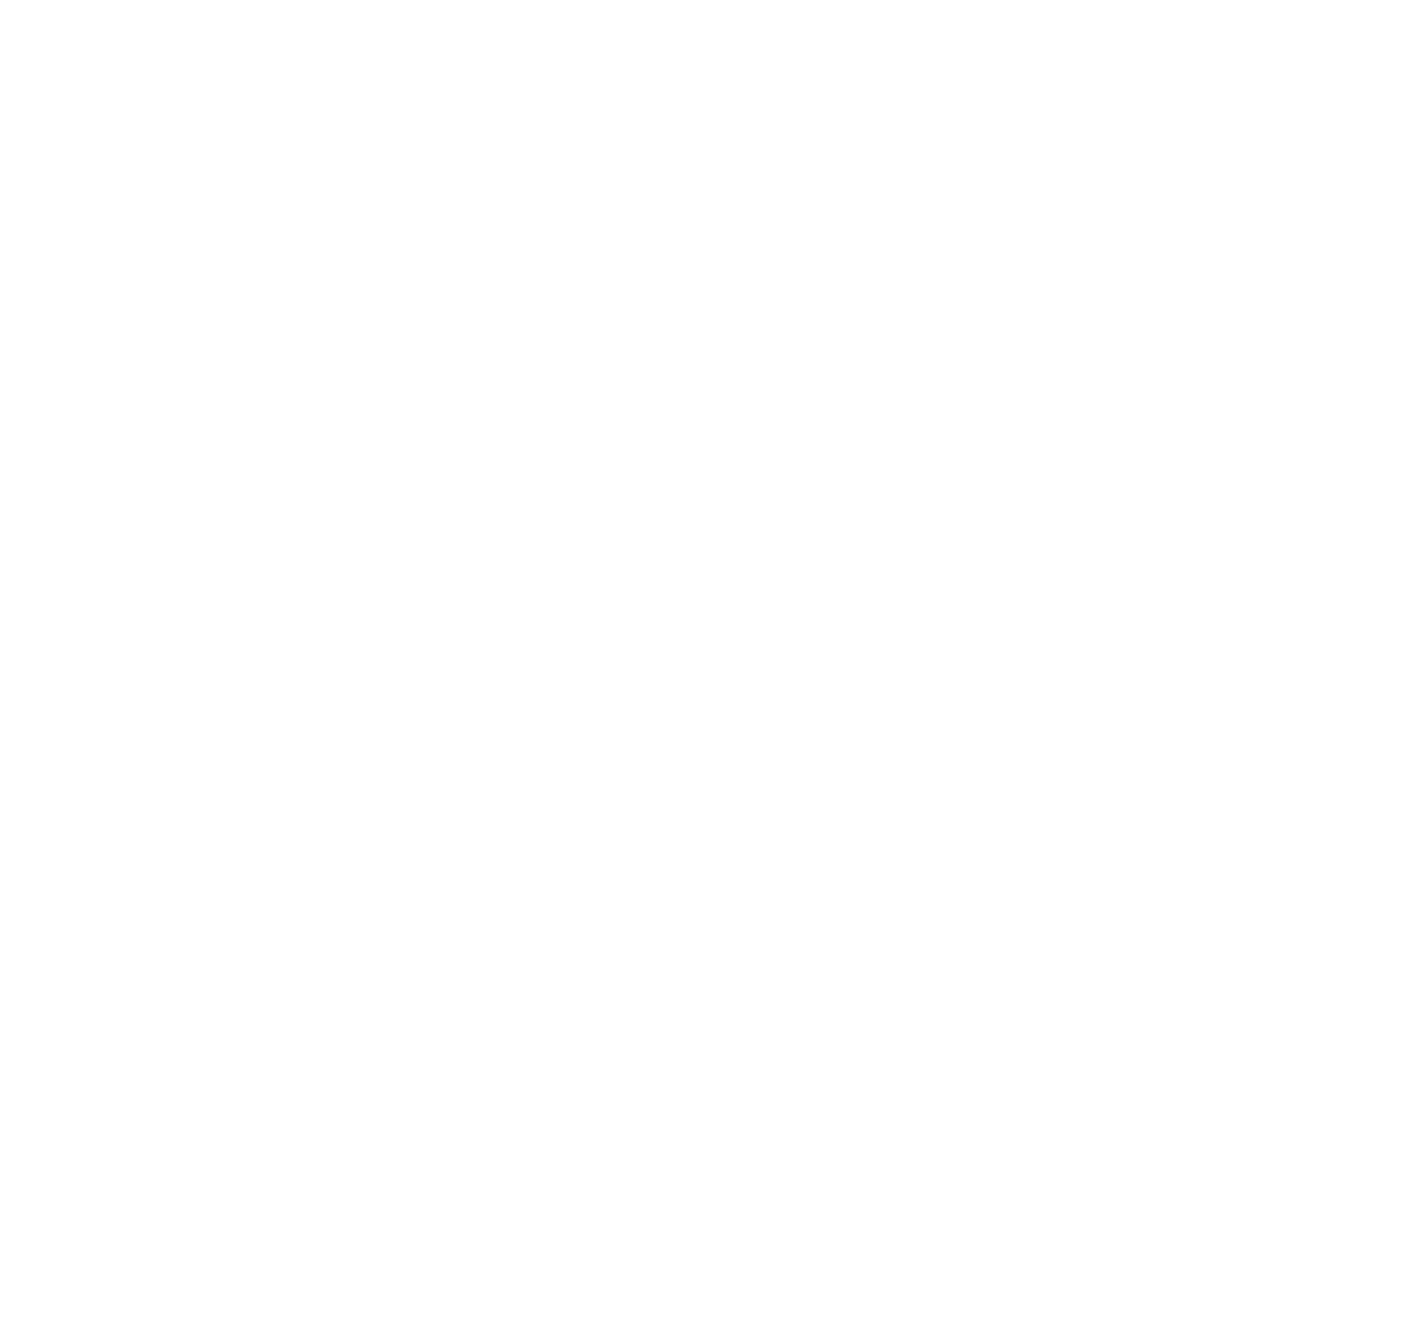
\includegraphics[width=\textwidth]{img/intro-0}}
        \only<2>{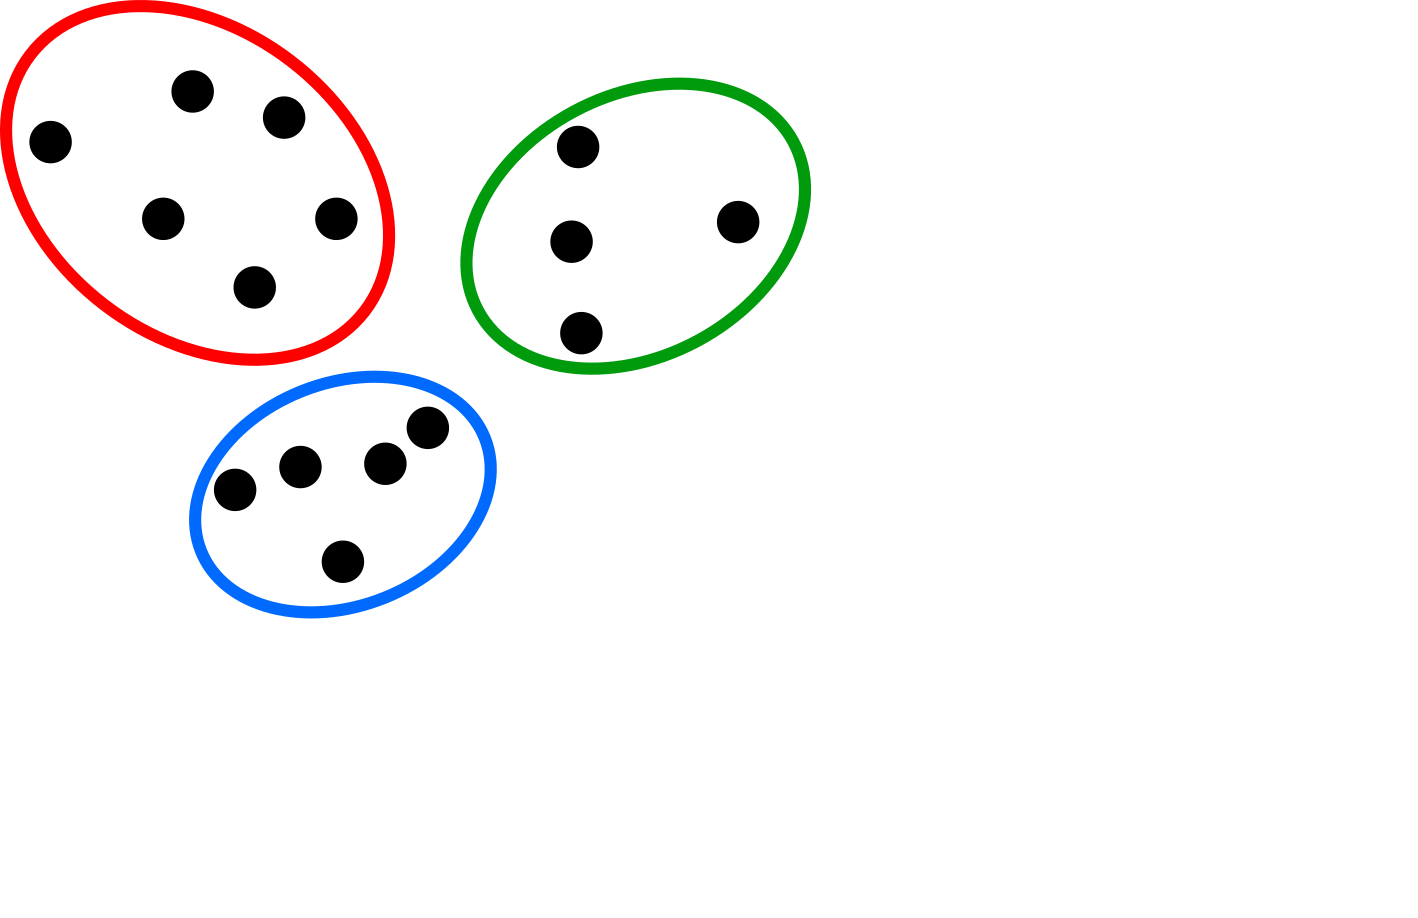
\includegraphics[width=\textwidth]{img/intro-1}}
        \only<3>{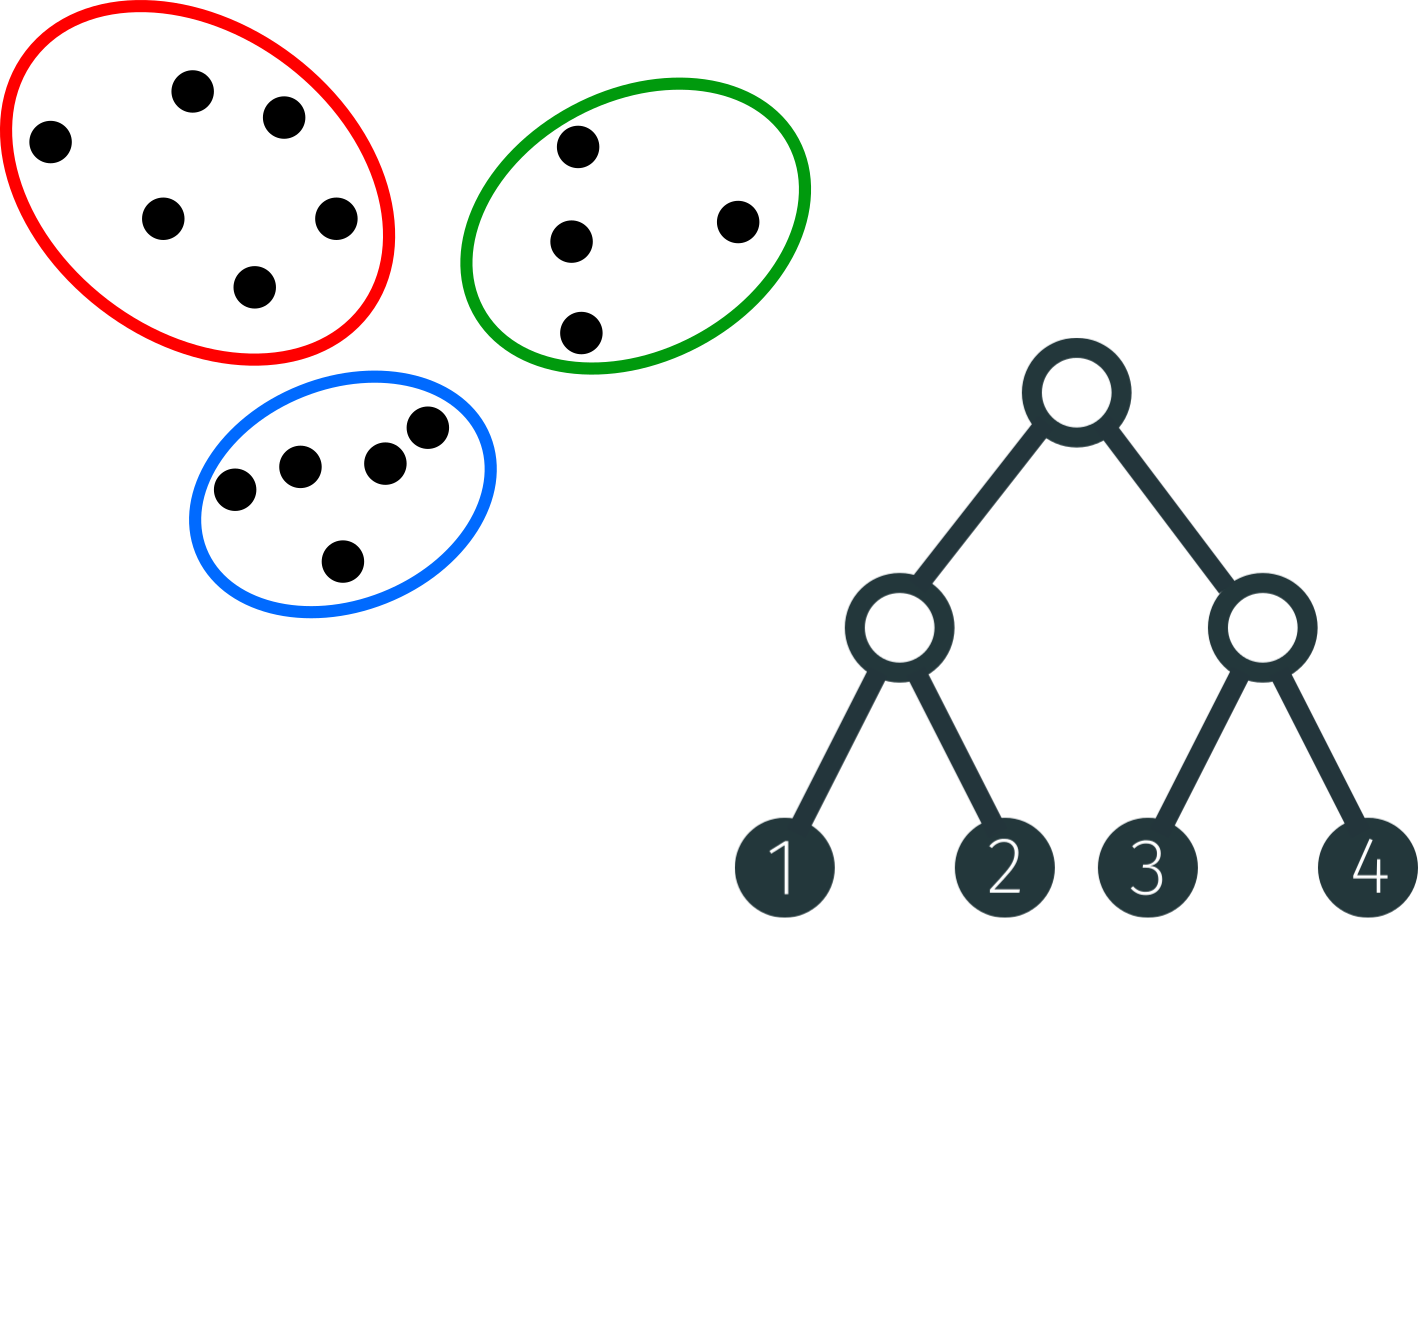
\includegraphics[width=\textwidth]{img/intro-2}}
        \only<4->{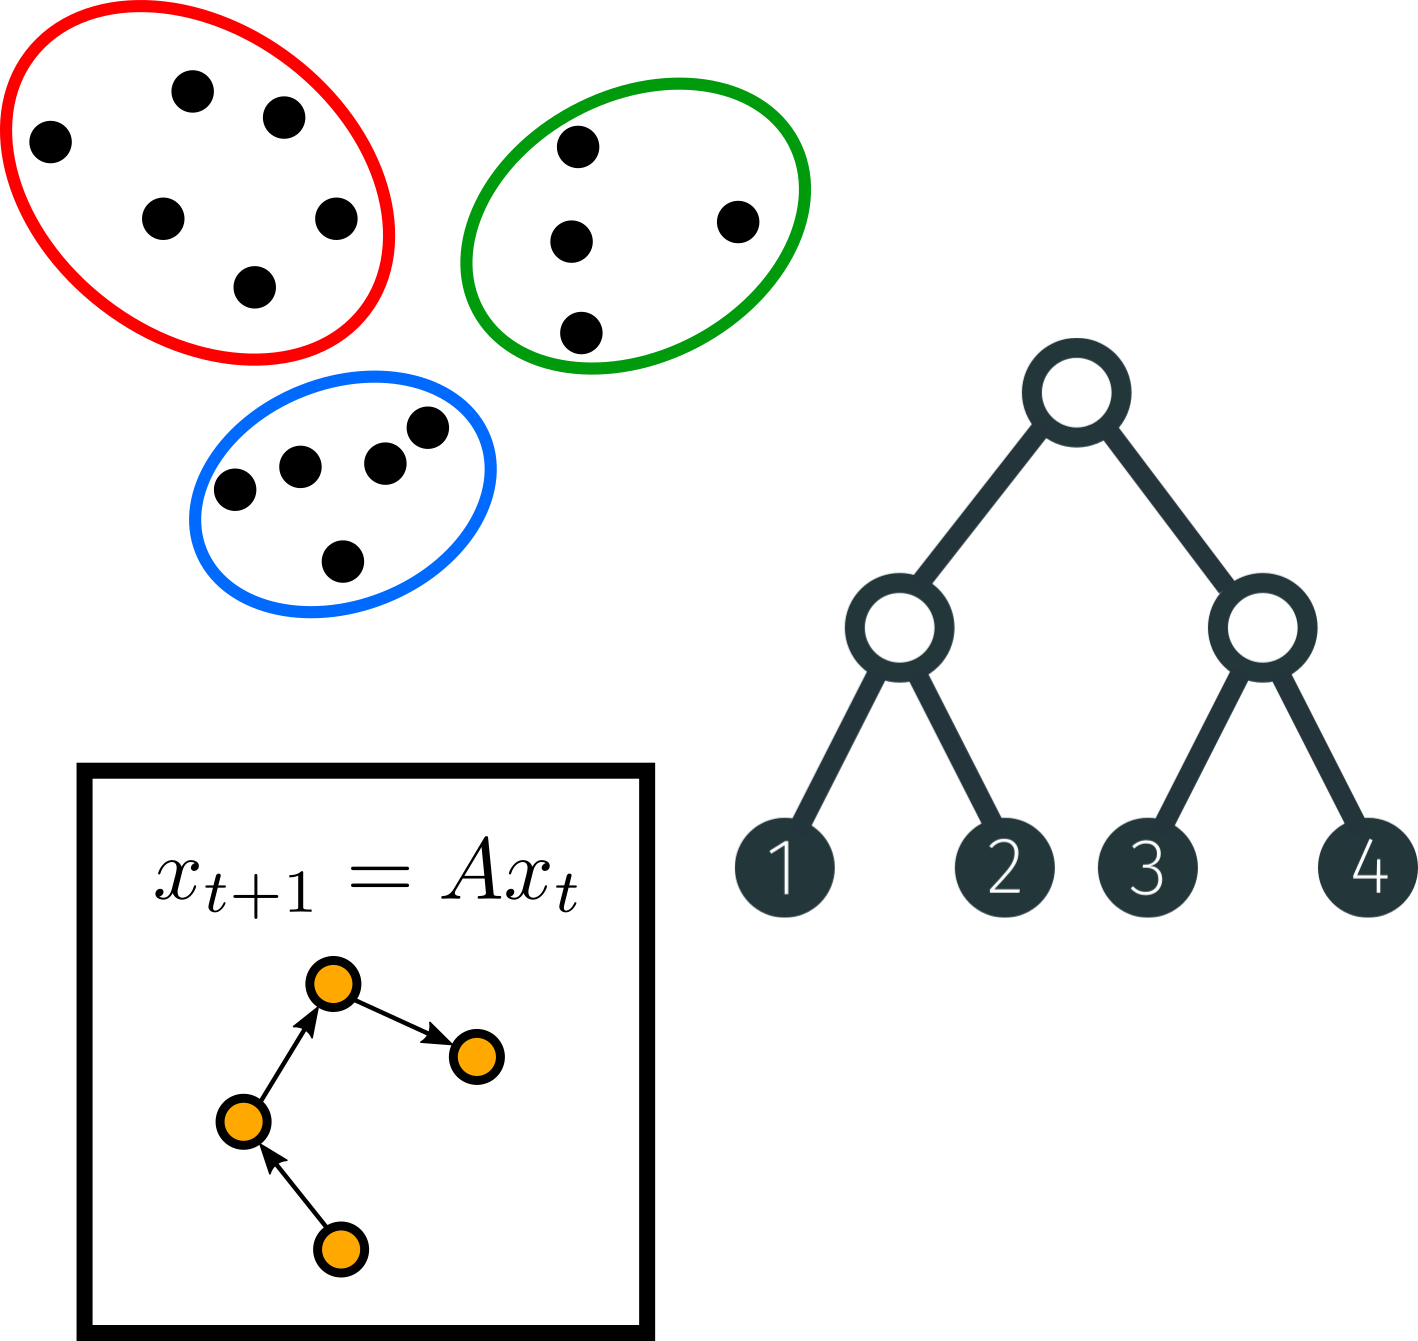
\includegraphics[width=\textwidth]{img/intro-3}}
        \end{center}
      \end{overlayarea}
    \end{column}
    \begin{column}{0.5\textwidth}
      \begin{overlayarea}{\textwidth}{5cm}
        \centering
        \Large \textbf{Embedding} \\ \vspace{10pt}
        \only<5->{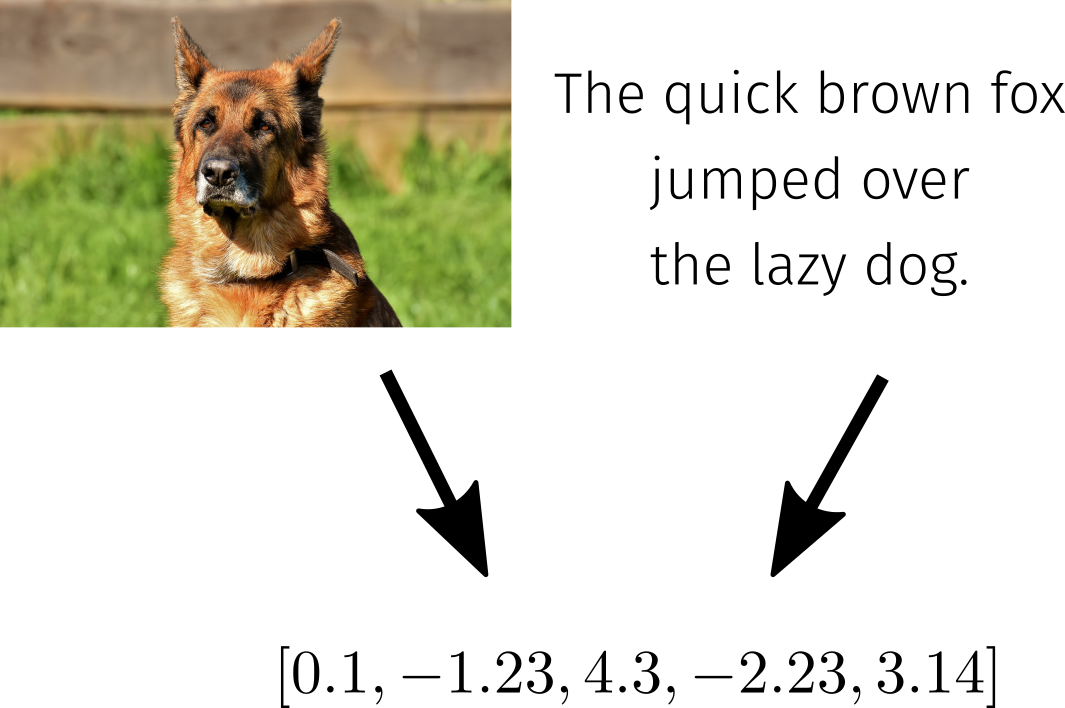
\includegraphics[width=\textwidth]{img/intro-right-1}}
      \end{overlayarea}
    \end{column}
  \end{columns}
\end{frame}

\begin{frame}{Bayesian unsupervised learning}
  \centering
  \begin{figure}
    \centering
    \pause
    \begin{subfigure}[t]{0.20\textwidth}
        \centering
        \includegraphics{tikz/gmm}
        \caption{Gaussian mixture model}
    \end{subfigure}
    \pause
    \hfill
    \begin{subfigure}[t]{0.20\textwidth}
        \centering
        \includegraphics{tikz/tmc}
        \caption{Bayesian hierarchical clustering}
    \end{subfigure}
    \pause
    \hfill
    \begin{subfigure}[t]{0.20\textwidth}
        \centering
        \includegraphics{tikz/lds}
        \caption{Bayesian linear dynamical system}
    \end{subfigure}
    \pause
    \begin{subfigure}[t]{0.20\textwidth}
        \centering
        \includegraphics{tikz/vae}
        \caption{Variational autoencoder}
    \end{subfigure}
  \end{figure}
\end{frame}

\begin{frame}{Research overview}
  \centering
  \multiinclude[<+>][format=png, graphics={width=0.8\textwidth}]{img/overview}
\end{frame}

\section{Bayesian structure learning}

\begin{frame}{Structure learning}
  \centering
  What is structure learning?

  \pause
  \centering
  \begin{figure}
    \centering
    \pause
    \begin{subfigure}[t]{0.27\textwidth}
        \centering
        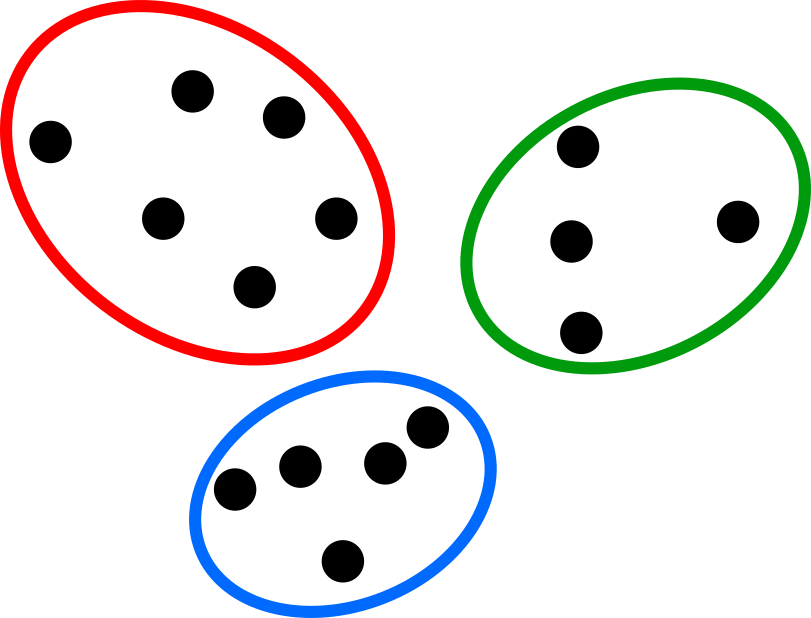
\includegraphics[width=\textwidth]{img/clustering}
    \end{subfigure}
    \pause
    \hfill
    \begin{subfigure}[t]{0.27\textwidth}
        \centering
        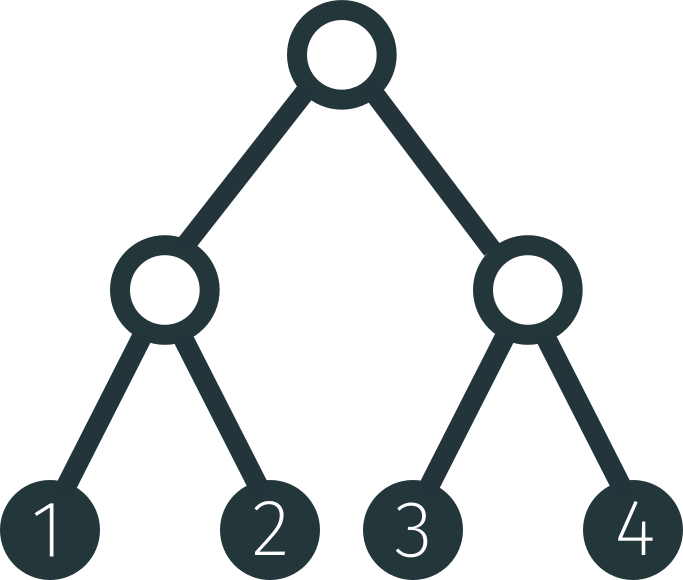
\includegraphics[width=\textwidth]{img/tree-1234-balanced}
    \end{subfigure}
    \pause
    \hfill
    \begin{subfigure}[t]{0.27\textwidth}
        \centering
        \includegraphics[width=\textwidth]{img/lds}
    \end{subfigure}
  \end{figure}
  \pause
  Structure learning seeks out intuitive relationships in data.

\end{frame}

\begin{frame}{Challenge: ambiguity}
  \centering
  Consider the clustering scenario.

  \multiinclude[<+->][format=png, start=0, end=4]{img/ambiguous-bayes}

  \only<6>{A Bayesian approach models this ambiguity}

\end{frame}

\begin{frame}{Can we do better?}
  \centering

  \only<-3>{
    \vspace{20pt}
    \multiinclude[<+-3>][format=png]{img/cluster-interaction}
    \vspace{20pt}
  }

  \only<4>{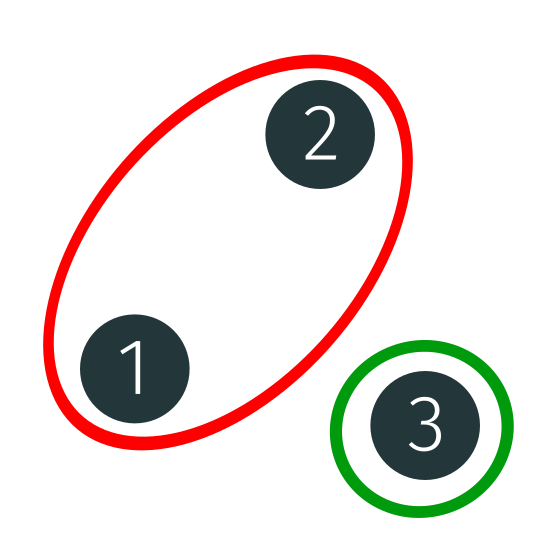
\includegraphics{img/ambiguous-cluster3-2}}

  \onslide<3-4>{User provides constraint $1$ must link with $2$.}

\end{frame}

\begin{frame}{Interactive structure learning}

  \multiinclude[<+->][graphics={width=\textwidth}, format=png, start=1]{img/structure-interaction}

  \onslide<2->{Algorithm provides a structure $S$}
  \onslide<3->{and human provides a constraint $c$}

\end{frame}

\begin{frame}{Bayesian interactive structure learning}
  \centering
  How are these problems framed in the Bayesian setting?

  \pause
  \vspace{10pt}

  \only<2>{\includegraphics{tikz/structure}}

  \only<3>{\includegraphics{tikz/interactive-structure}}

  \only<2>{We are interested in $p(S | \bm{y})$}

  \only<3>{We are interested in $p(S | \bm{y}, c)$}

\end{frame}

\begin{frame}{Current work}
  \begin{itemize}
    \pause
    \item Flat clustering - \cite{wat}
    \pause
  \item \structure<3>{Hierarchical clustering - Vikram and Dasgupta, ICML 2015}
  \end{itemize}
\end{frame}

\begin{frame}{Interactive hierarchical clustering}
  \begin{center}
    \includegraphics<1>[width=\textwidth]{img/interaction-0}
    \includegraphics<2>[width=\textwidth]{img/interaction-1}
    \includegraphics<3>[width=\textwidth]{img/interaction-2}
    \includegraphics<4->[width=\textwidth]{img/interaction-3}
  \end{center}
  \begin{itemize}
    \item<4-> User provides a \alert{triplet}. $a$ and $b$
  should be in a subtree together without $c$.
    \item<5-> We show the user the induced tree on the subset of the data $T|_S$.
  \end{itemize}
\end{frame}

\begin{frame}{Bayesian hierarchical clustering}
  We desire a probability distribution over all possible
  trees that explain the data.

  \begin{center}
    \includegraphics<2>[width=0.7\textwidth]{img/3-cluster-distribution.png}
    \includegraphics<3>[width=0.7\textwidth]{img/3-cluster-linear-distribution.png}
  \end{center}
\end{frame}

\begin{frame}{Bayesian hierarchical clustering}
  Define a generative model for the data.
  \begin{itemize}
    \item<1->   Prior distribution $P(T)$, (Dirichlet diffusion tree,
      Kingman's coalescent)
    \item<3->   Likelihood model $P(\theta | T), P(X | T, \theta)$, (Brownian motion,
      Dirichlet-multinomial diffusion)
  %\begin{center}
    %\includegraphics<2>[width=\textwidth]{img/diffusion-1}
    %\includegraphics<3>[width=\textwidth]{img/diffusion-2}
    %\includegraphics<4>[width=\textwidth]{img/diffusion-3}
    %\includegraphics<5>[width=\textwidth]{img/diffusion-4}
  %\end{center}
  \end{itemize}

  \begin{center}
    \includegraphics<2-3>[width=\textwidth]{img/tree-data-0}
    \includegraphics<4>[width=\textwidth]{img/tree-data-1}
  \end{center}

\end{frame}

\begin{frame}{Inference}
  We are interested in the posterior distribution
  $P(T | X)$, which we compute
  via approximate methods like Metropolis-Hastings.

  \uncover<2->{A popular proposal distribution is \alert{subtree-prune
  and regraft} (SPR).}

  \begin{center}
    \includegraphics<3>[width=\textwidth]{img/spr-1}
    \includegraphics<4>[width=\textwidth]{img/spr-2}
    \includegraphics<5->[width=\textwidth]{img/spr-3}
  \end{center}

  \uncover<6->{Parameters $\theta$ can be sampled via Gibbs sampling
  or integrated out via belief propagation.}

\end{frame}

\begin{frame}{Incorporating triplet feedback}

  Recall the interaction model.

  \begin{center}
    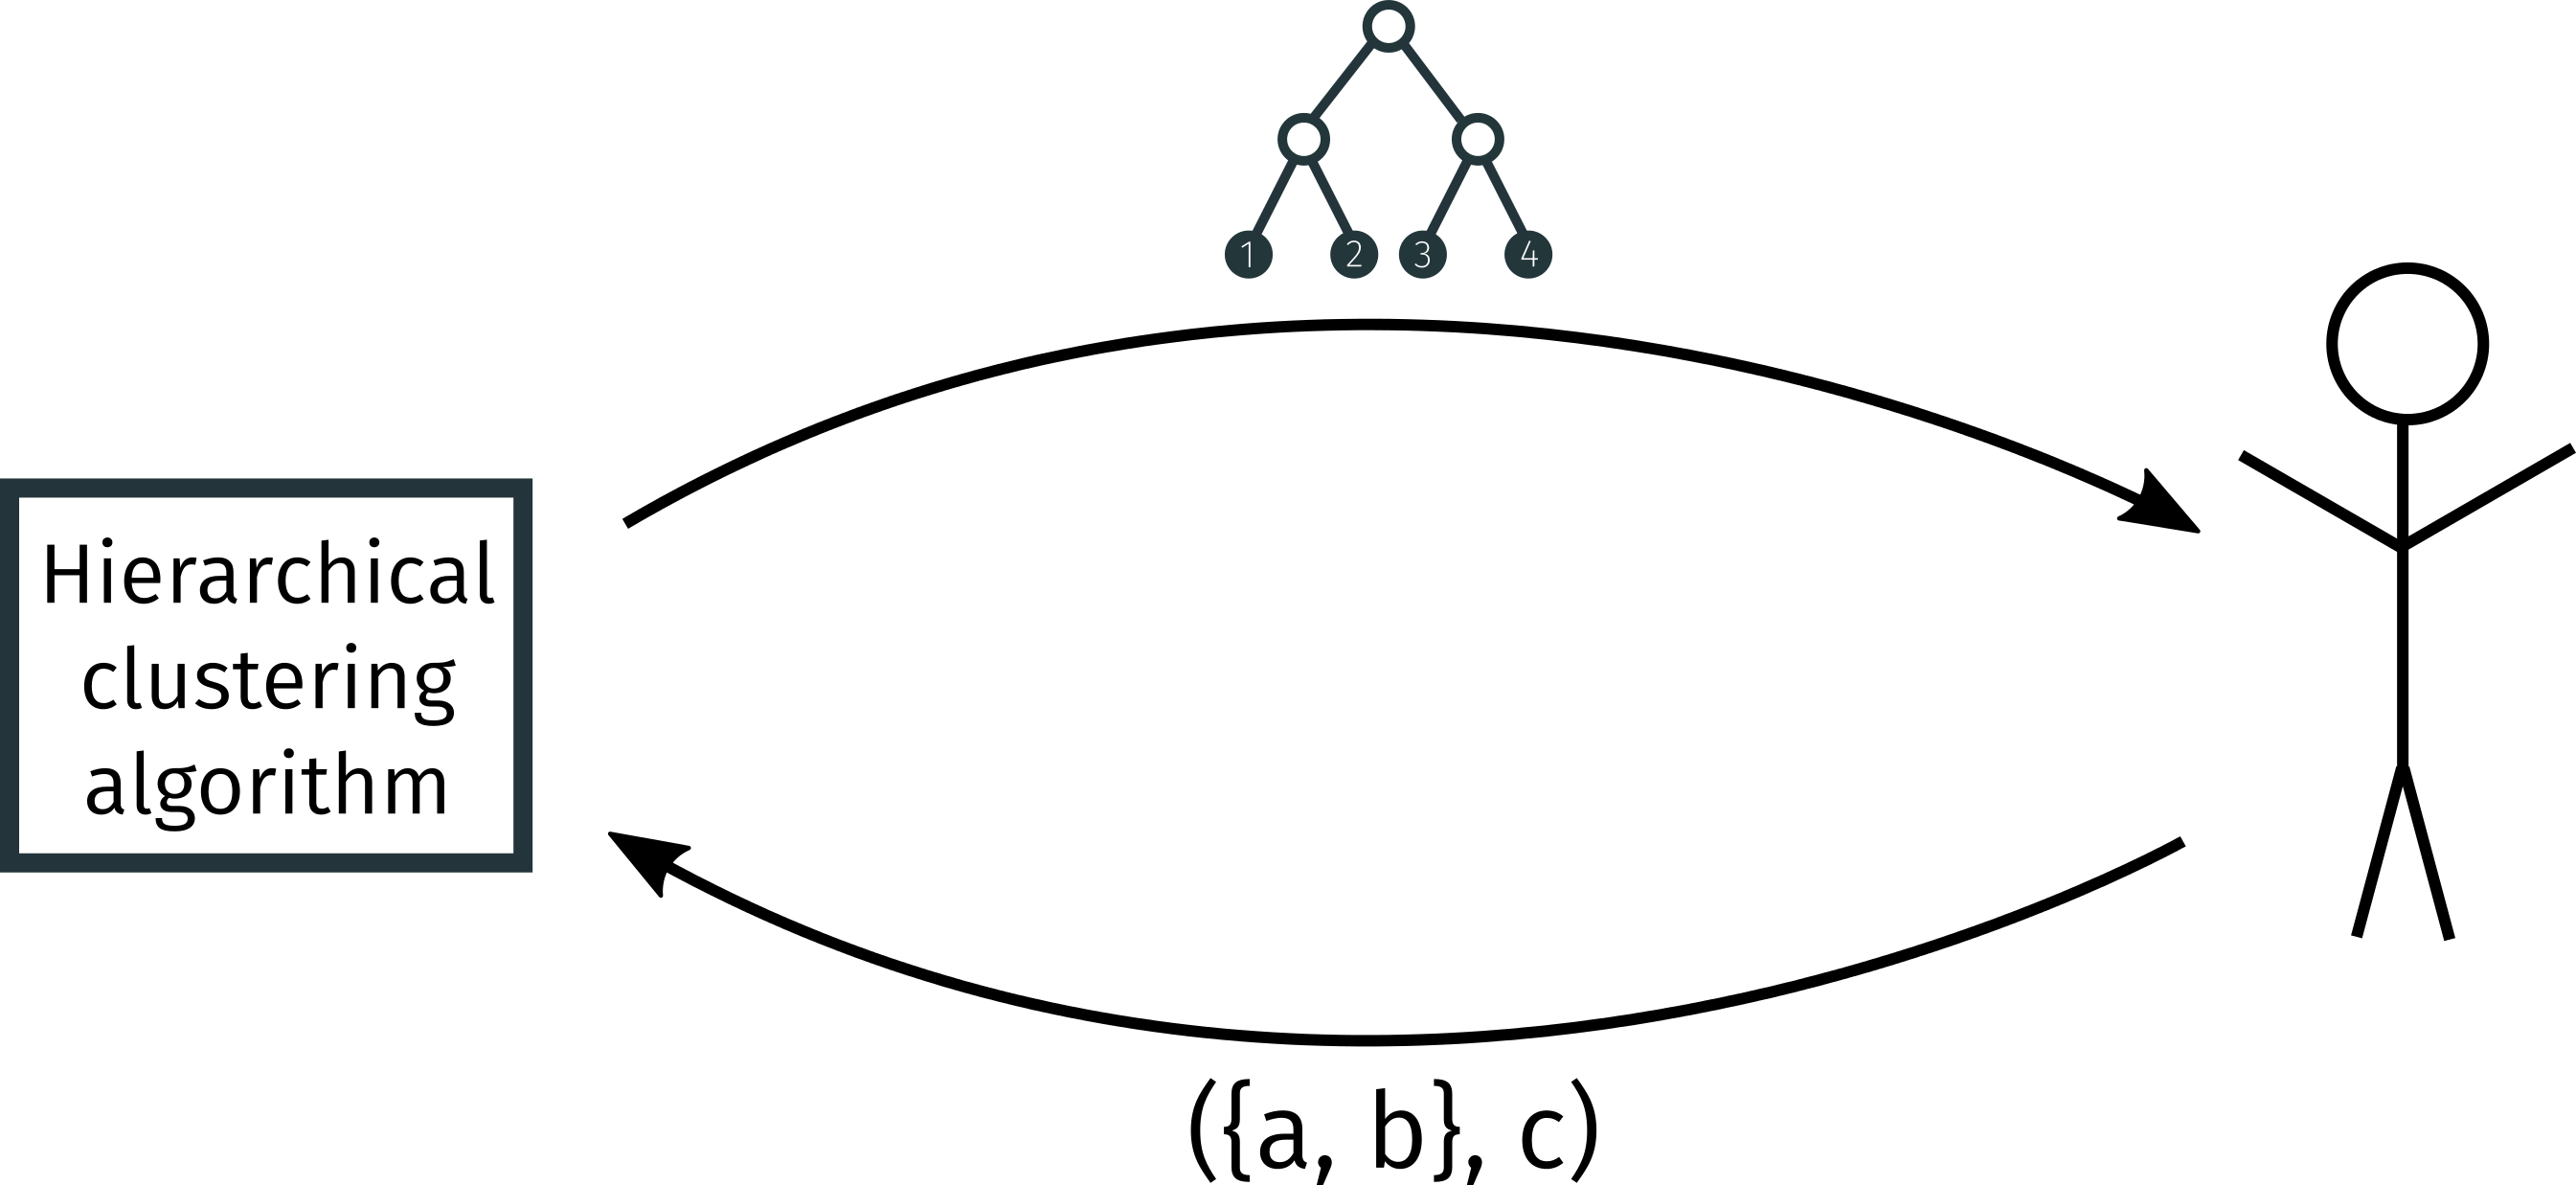
\includegraphics[width=0.7\textwidth]{img/interaction-3}
  \end{center}
  \pause

  \textbf{Idea:}  enforce triplet constraints with
  modified SPR move

  \pause

  \begin{center}
    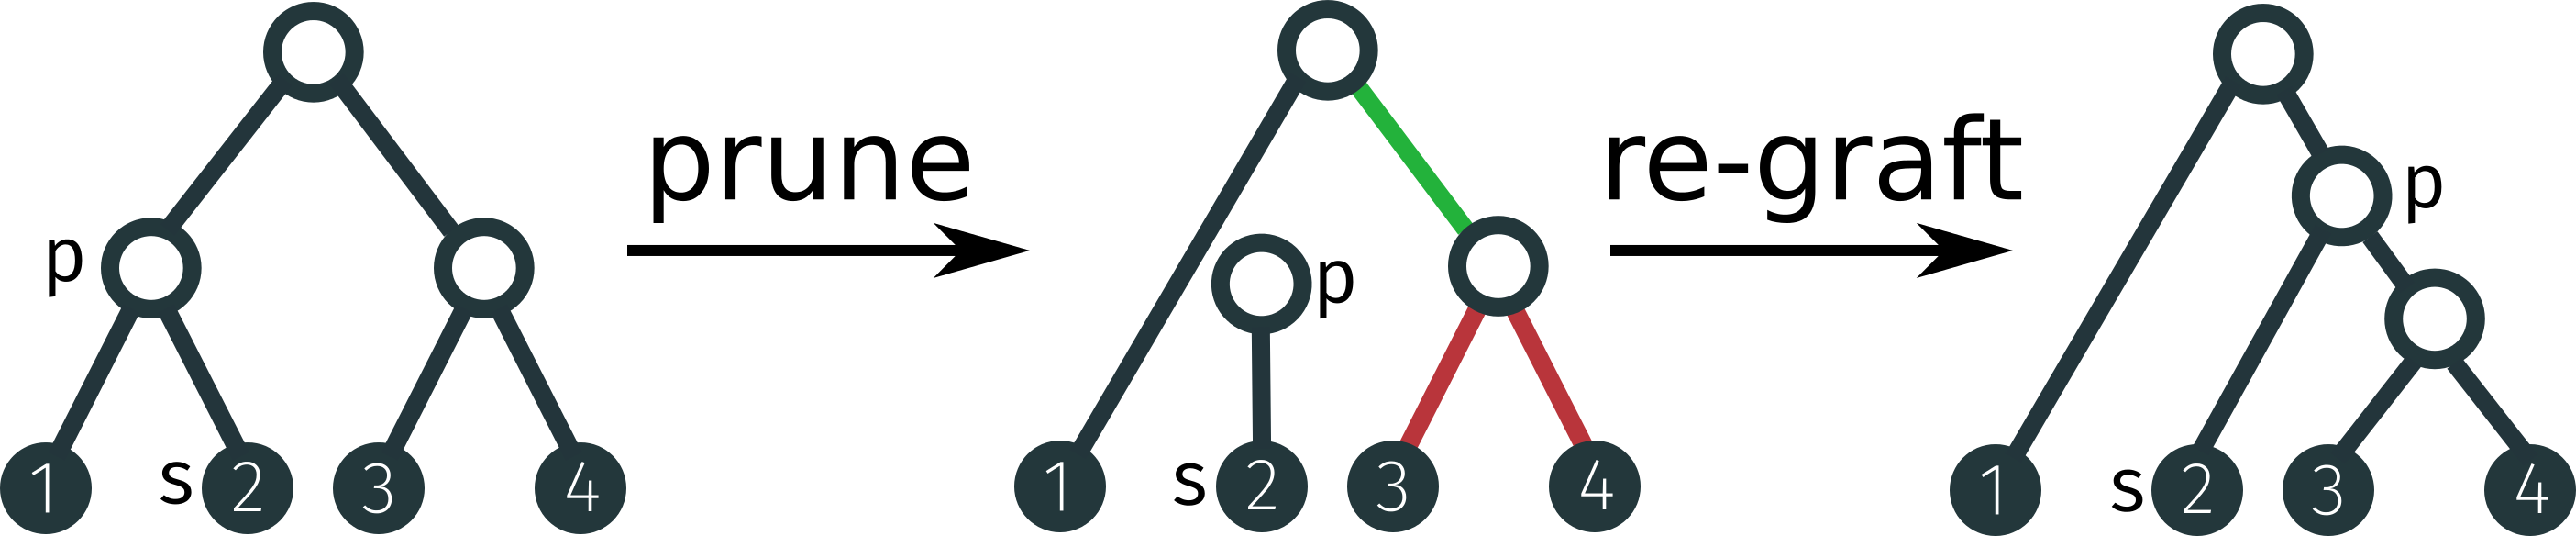
\includegraphics[width=\textwidth]{img/cspr-animation}
  \end{center}
\end{frame}

\iffalse
\begin{frame}{Intelligent subset queries}

  Recall the interaction model.

  \begin{center}
    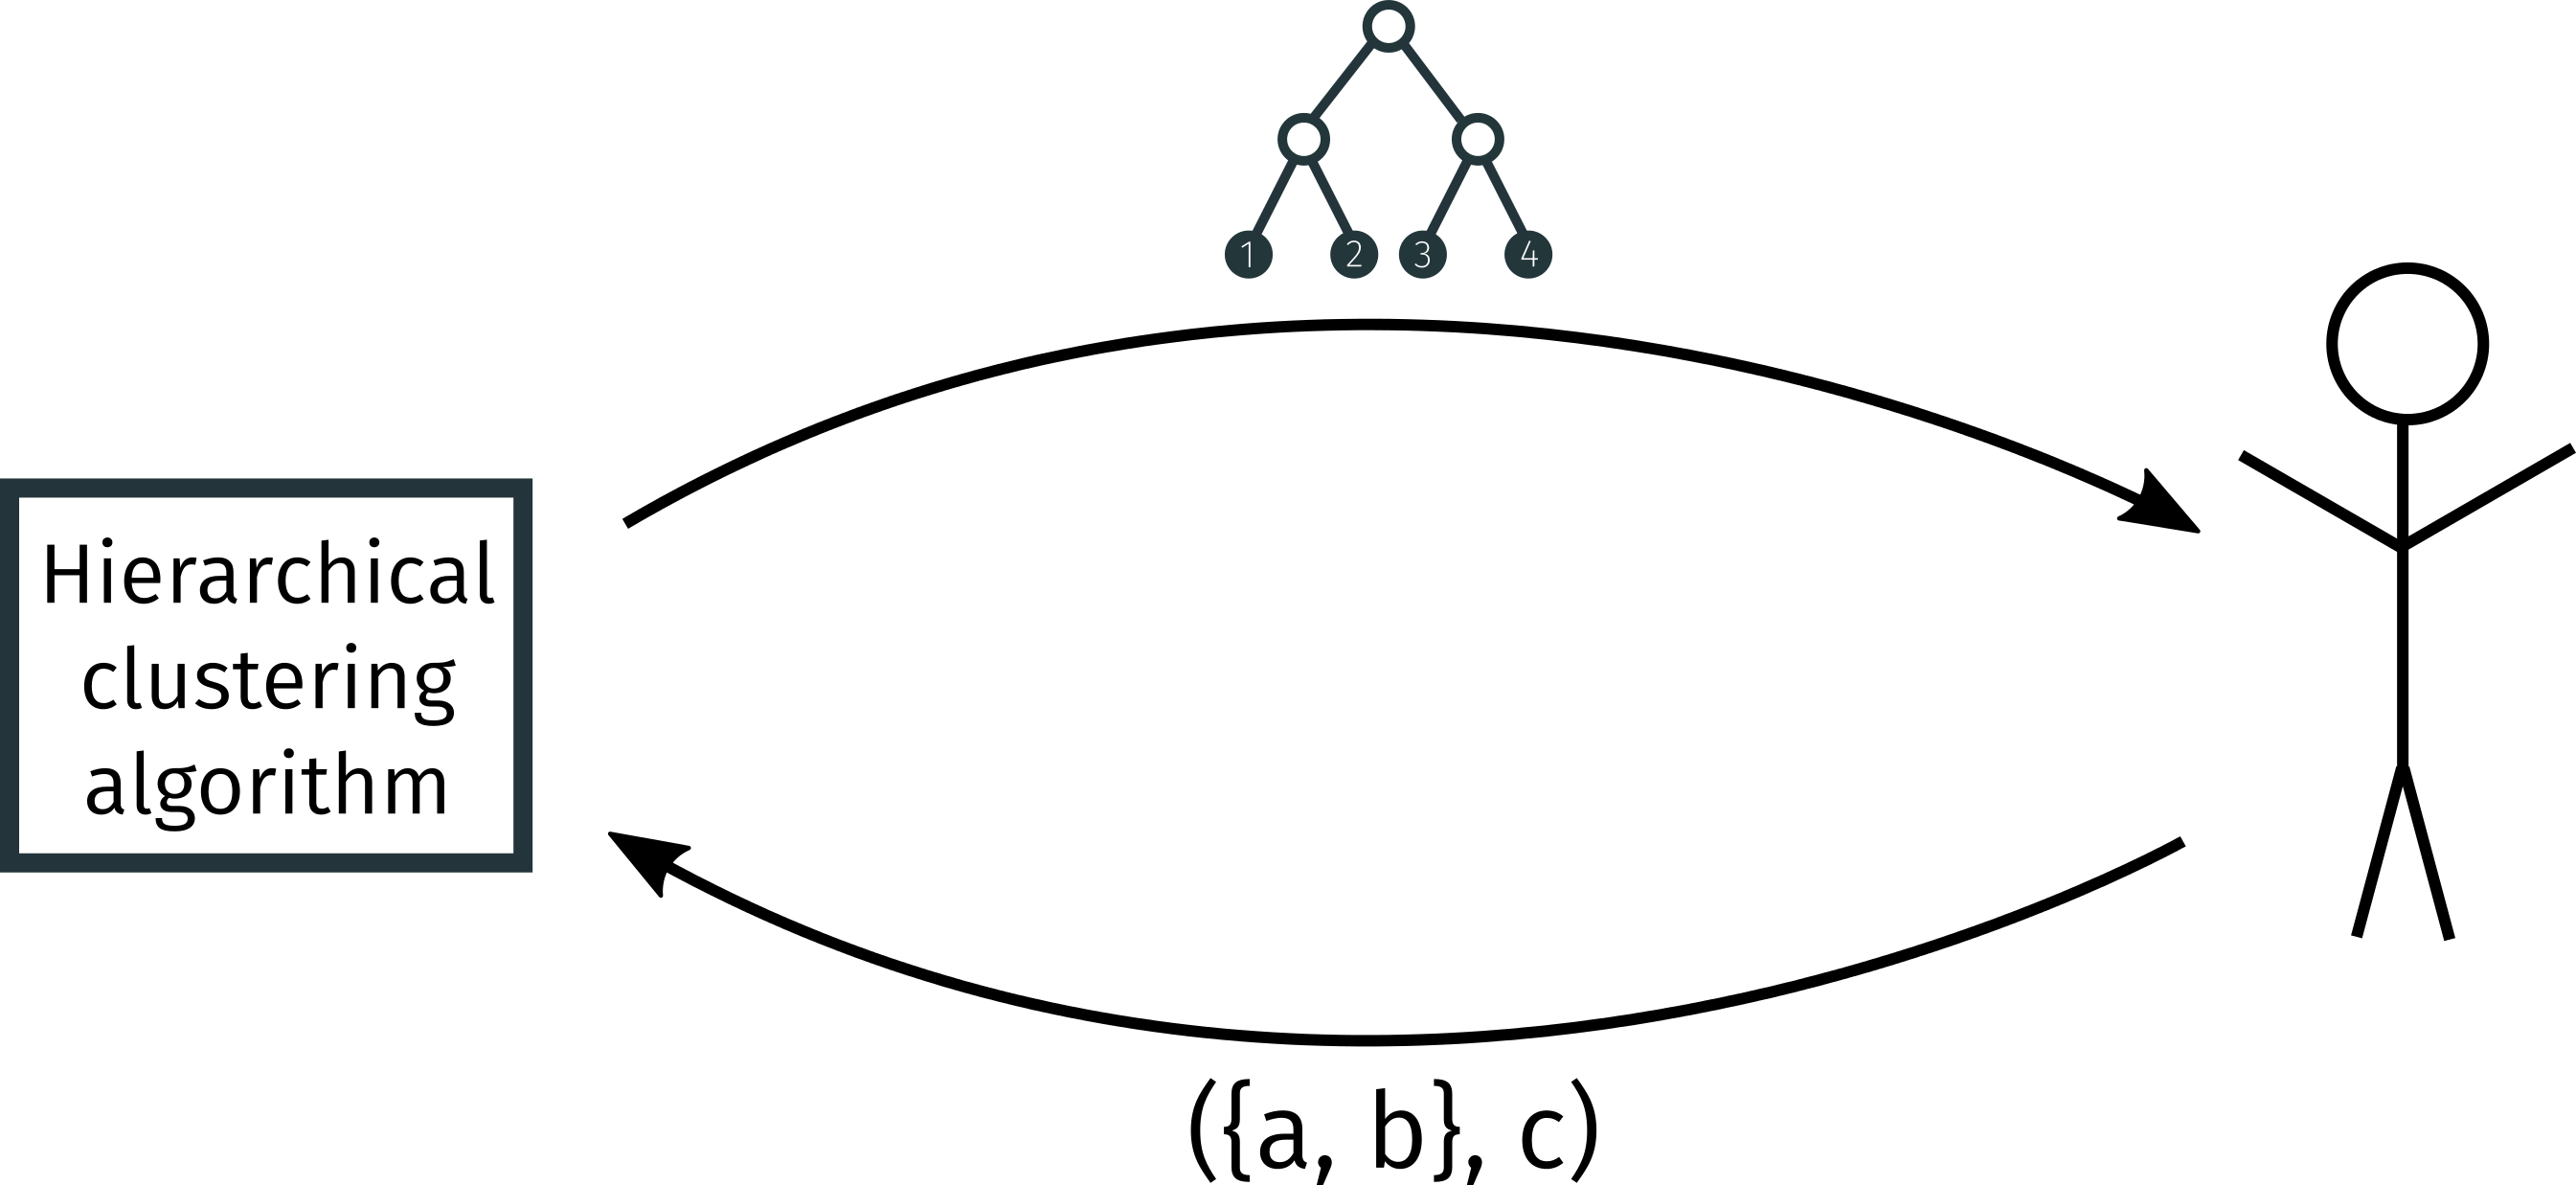
\includegraphics[width=\textwidth]{img/interaction-3}
  \end{center}

  \pause

  %We pick a subset of data $S$ and show a user the candidate tree
  %restricted to $S$, $T|_S$.

  %\pause

  \textbf{Idea:}  pick subsets that have high variance
  under the posterior distribution

\end{frame}

\begin{frame}{Measuring subtree variance}

    First, sample $N$ trees from posterior distribution.

  \pause

 \metroset{block=fill}
  \begin{block}{Definition: tree distance variance (TDV)}
    Given a subset of data $S$ and tree samples $\mathcal{T} = T_1, \ldots, T_N$,
    \begin{align}
      \mathrm{TDV}(S, \mathcal{T}) = \max_{i, j \in S}  \mathrm{Var}_{T \in \mathcal{T}}\left[\texttt{tree-dist}_{T|S}(i, j)\right]
    \end{align}
  where $\texttt{tree-dist}_T$ is the number of edges needed to get from leaf $i$ to leaf $j$
  in tree $T$.
  \end{block}

  \pause

Instantiate $L$ subsets randomly and pick the one with the highest variance.

\end{frame}
\fi

\begin{frame}{IBHC results}
  \centering
  \frame{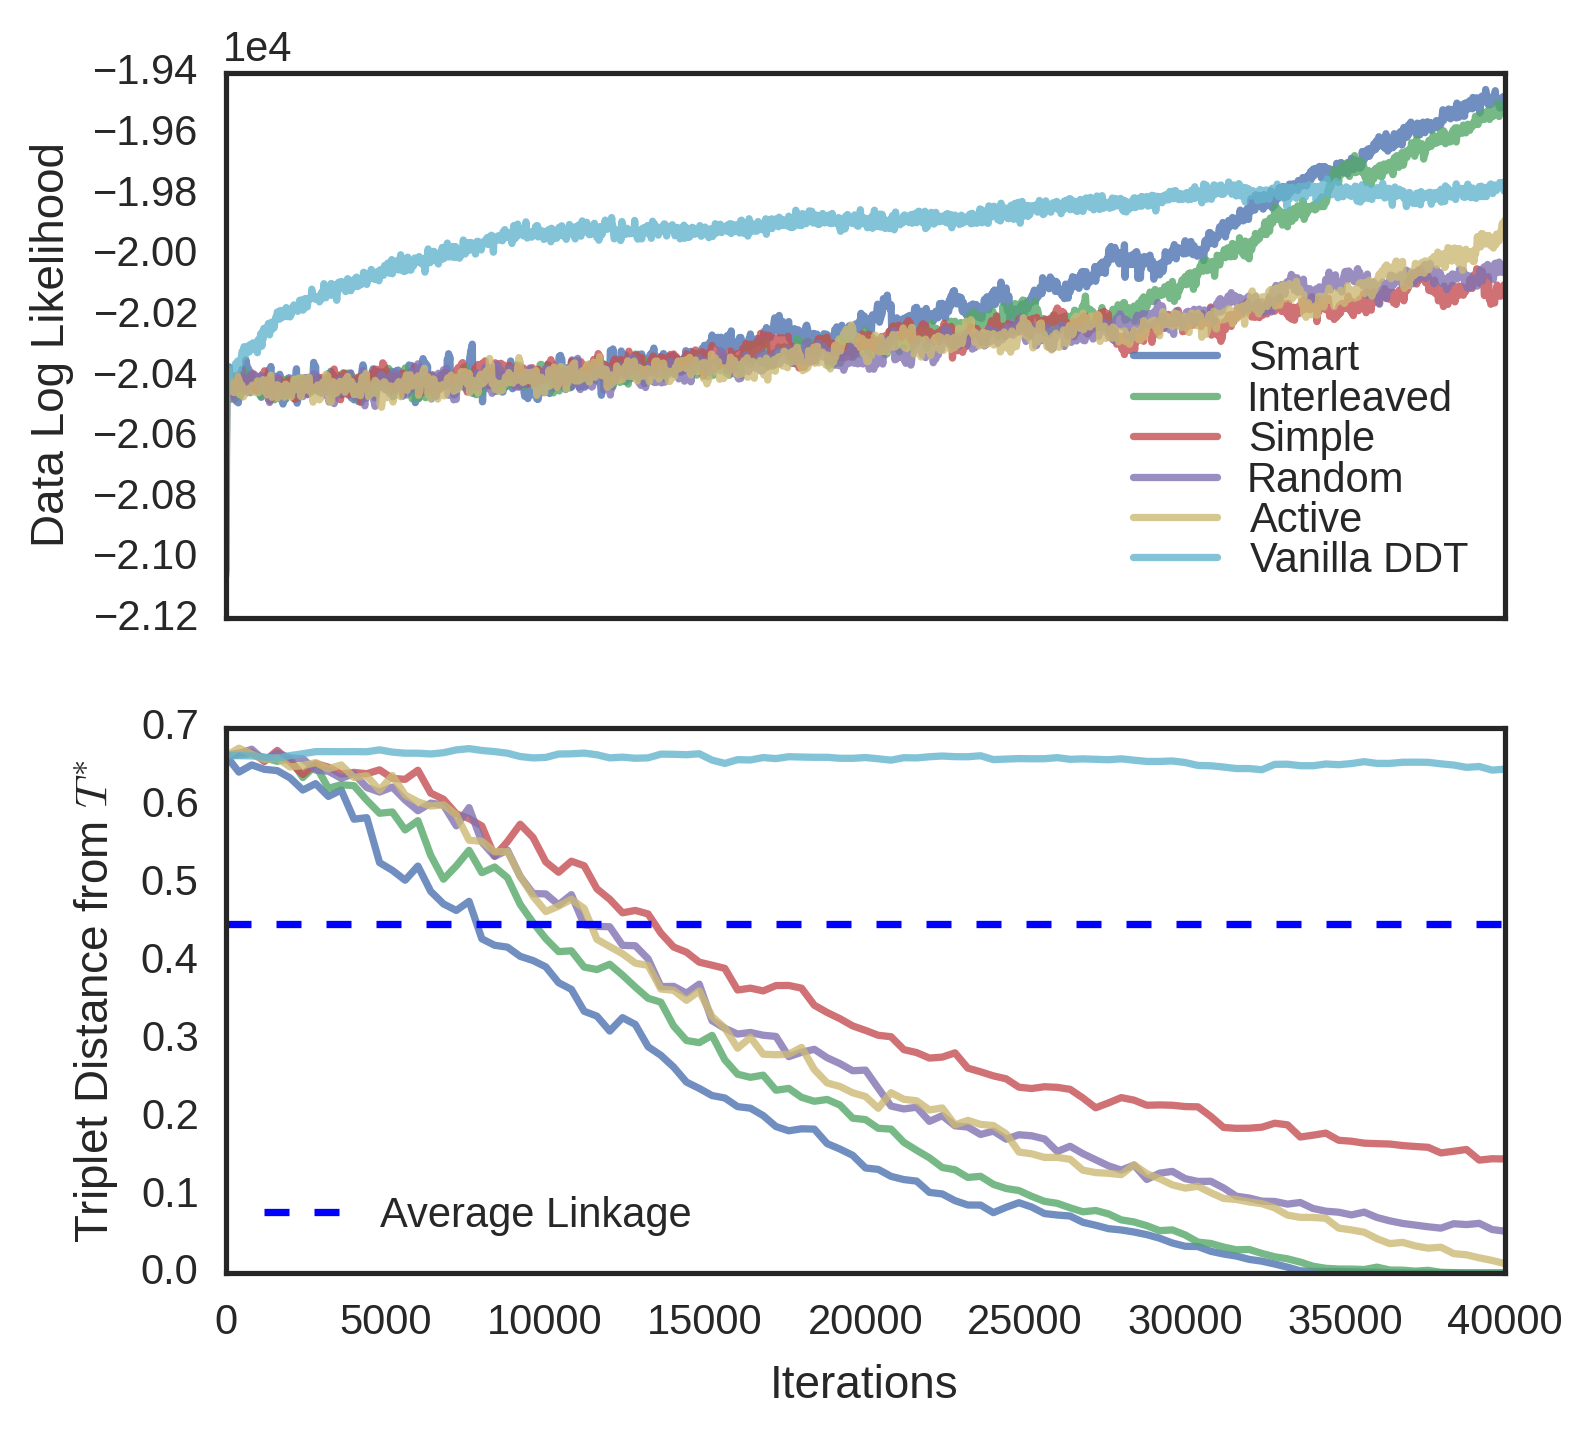
\includegraphics[width=0.8\textwidth]{img/trees/MNIST-result}}
\end{frame}

\section{Bayesian embedding learning}

\begin{frame}{Bayesian embedding learning}
  \centering
  What's the difference between embedding and structure learning?
  \pause
  \begin{center}
    \begin{columns}
      \begin{column}{0.3\textwidth}
        \includegraphics{tikz/structure}
      \end{column}
    \pause
      \begin{column}{0.3\textwidth}
        \includegraphics{tikz/embedding}
      \end{column}
    \end{columns}
  \end{center}
\end{frame}
\begin{frame}{Variational autoencoder}
  The VAE is a generative model for data.
  \begin{align*}
    x_i &\sim  \N(0, I) \\
    y_i &\sim  \N(\mu_\gamma(x_i), \Sigma_\gamma(x_i))
  \end{align*}
  where $\mu_\gamma$ and $\Sigma_\gamma$ are neural networks parameterized by $\gamma$.

  \pause
  \centering
  \includegraphics{tikz/vae}
  \pause
   
  How do we do inference?
  \alert<+>{Variational inference}
\end{frame}

\begin{frame}{Variational inference at a high level}
  For models where we can't compute
  the posterior analytically, \textbf{variational inference}
  is a viable approach.

  \pause
    Consider a latent variable model with global variables
    $\theta$, local variables $x$ and observations $y$. Our desired
    posterior is $p(\theta, x | y)$

    \pause
    \textbf{Strategy}: convert inference into optimization
    \begin{itemize}
        \pause
      \item Instantiate \emph{variational distribution} $q_\phi(\theta, x)$
        where $\phi$ are free parameters
        \pause
      \item Define loss $\textrm{KL}(q_\phi(\theta, x)\|p(\theta, x | y))$
        \pause
      \item Minimize loss $\phi^* = \argmin_\phi \textrm{KL}(q_\phi(\theta, x)\|p(\theta, x | y))$
    \end{itemize}
    \pause
    If $q(\theta, x)$ is sufficiently expressive,
    it can approximate $p(\theta, x | y)$ quite well.
\end{frame}

\begin{frame}{KL-divergence}
  Kullback-Leibler (KL) divergence
  is a measure of how far one probability distribution
  is from another.

  \pause
  For distributions $q(x)$ and $p(x)$,
  \begin{align*}
    \textrm{KL}(q(x)\|p(x)) = \int q(x)\log \frac{q(x)}{p(x)}dx = \E_{q(x)}\left[\log\frac{q(x)}{p(x)}\right]
  \end{align*}

  \pause
  \textbf{Properties:}
  \begin{itemize}
    \item $\textrm{KL}(q(x)\|p(x)) = 0$ if $q(x) = p(x)$.
    \item Asymmetric
  \end{itemize}

\end{frame}

\begin{frame}{Evidence lower bound}
  In general, we cannot even compute $KL(q(\theta, x)\|p(\theta, x | y))$
  because
  we don't know the posterior $p(\theta, x | y)$.

  \pause
  We can rewrite the KL divergence as
  \begin{align*}
    \KL(q(\theta, x)\|p(\theta, x|y)) &= \int q(\theta, x)\log\frac{q(\theta, x)}{p(\theta, x | y)}d\theta, x \\
    %&= \int q(\theta, x) \left(\log q(\theta, x) - \log p(\theta, x | y)\right)d\theta, x \\
    %&= \int q(\theta, x) \left(\log q(\theta, x) - \log \frac{p(\theta, x, y)}{p(y)}\right)d\theta, x \\
    %&= \int q(\theta, x) \left(\log q(\theta, x) - \log p(\theta, x, y) + \log p(y)\right)d\theta, x \\
              &= \log p(y) - \E_{q(\theta, x)}\left[\log\frac{p(y, \theta, x)}{q(\theta, x)}\right]
  \end{align*}

  \pause
  and maximize the \emph{evidence lower bound} (ELBO)
  \begin{align*}
    \L[q(\theta, x)] &= \E_{q(\theta, z)}\left[\log\frac{p(y, \theta, x)}{q(\theta, x)}\right]
  \end{align*}
\end{frame}
\begin{frame}{Variational autoencoder}
  \textbf{Basic strategy:} gradient-based variational inference

  \pause

  \begin{itemize}
    \item Pick $q_\phi(x | y)$ to be a \emph{neural network} parameterized by $\phi$ (both differentiable and sampleable)
  \end{itemize}

  \pause
  Let $r_\phi(y)$ be a neural network (with weights $\phi$)
  that outputs the parameters to a distribution, for example Gaussian.
  \begin{align*}
    q_\phi(x | y) = \N(r_\phi(y))
  \end{align*}

  \pause

  %\begin{itemize}
    %\item Use the reparametrization trick to lower variance of gradients
  %\end{itemize}
  \pause
  Goal: learn the weights for the two neural networks $(\mu_\gamma(x), \Sigma_\gamma(x))$ and $r_\phi(y)$
  via SGD on the ELBO.
  \pause
  \begin{align*}
    \L[q(x | y)] &= \E_{q(x | y)}\left[\log p(y, x) - \log q(x | y)\right]
  \end{align*}
\end{frame}

\begin{frame}{Monte-Carlo ELBO}
  We can't compute the ELBO because of the expectation w.r.t $q_\phi(z|x)$.
  \begin{align*}
    \L[q(x | y)] &= \E_{q(x | y)}\left[\log p(y, x) - \log q(x | y)\right]
  \end{align*}
  We can sample from $q$ however:
  \begin{align*}
    \hat{\L}[q(x | y)] &= \frac{1}{L}\sum_{l = 1}^L \left[\log p(y, x^{(l)}) - \log q(x^{(l)} | y)\right]
  \end{align*}
  Now, we can compute gradients.
  \begin{align*}
    \gamma^{(t + 1)} &\leftarrow \gamma^t - \rho \nabla_\gamma \hat{\L} \\
    \phi^{(t + 1)} &\leftarrow \phi^t - \rho \nabla_\phi \hat{\L} \\
  \end{align*}
\end{frame}

\begin{frame}{Recognition networks}


  \centering
  VAE uses neural networks as a tool for approximate inference.
  \pause
  Is this idea generalizable?
\end{frame}

\begin{frame}{Structured variational autoencoder}
  \centering
  \begin{columns}
    \begin{column}{0.3\textwidth}
      \includegraphics{tikz/lgmm}
    \end{column}
    \begin{column}{0.3\textwidth}
      \begin{align*}
        \pi &\sim \textrm{Dirichlet}(\alpha) \\
        \{\mu_k, \Sigma_k\}_{ik = 1}^K &\sim \NIW(\mu_0, \Sigma_0) \\
        \{z_i\}_{i = 1}^N &\sim \textrm{Categorical}(\pi) \\
        \{x_i\}_{i = 1}^N &\sim \N(\mu_{z_o}, \Sigma_{z_i})
      \end{align*}
    \end{column}
  \end{columns}
\end{frame}

\begin{frame}{Why SVAE?}

  \pause
  \begin{center}
    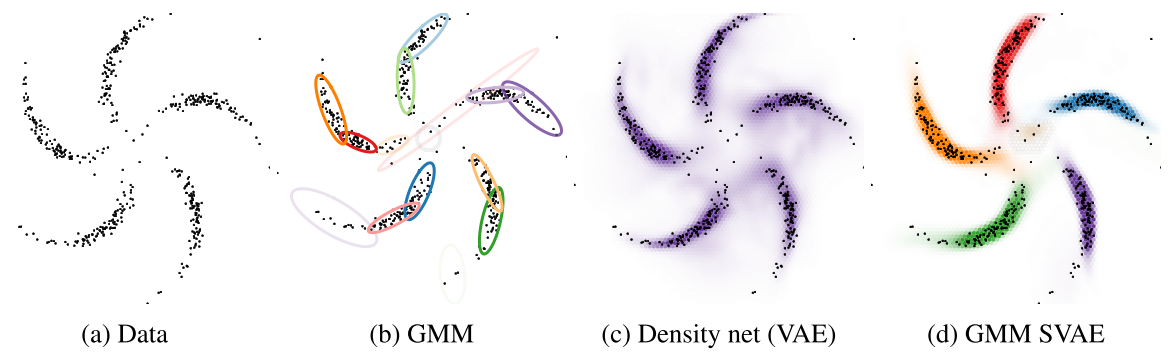
\includegraphics[frame,width=\textwidth]{img/svae-example}
  \end{center}

  \pause
  In this scenario, the SVAE enables modeling non-Gaussian cluster shapes \cite{svae}.
\end{frame}

\begin{frame}{Structured variational autoencoder}
  \centering
  \begin{columns}
    \begin{column}{0.3\textwidth}
      \includegraphics{tikz/lgmm}
    \end{column}
    \begin{column}{0.3\textwidth}
      \begin{align*}
        \pi &\sim \textrm{Dirichlet}(\alpha) \\
        \{\mu_k, \Sigma_k\}_{ik = 1}^K &\sim \NIW(\mu_0, \Sigma_0) \\
        \{z_i\}_{i = 1}^N &\sim \textrm{Categorical}(\pi) \\
        \{x_i\}_{i = 1}^N &\sim \N(\mu_{z_o}, \Sigma_{z_i})
      \end{align*}
    \end{column}
  \end{columns}
  \pause
  How do we do inference?
\end{frame}

\begin{frame}{Variational message passing}
  In variational inference for conjugate-exponential models,
  there is a simple graph algorithm, called \emph{variational message passing} (VMP).

  \begin{center}
    \multiinclude[graphics={width=0.5\textwidth},start=1]{img/vmp}
  \end{center}

\end{frame}

\iffalse
\begin{frame}{Messages}
  Remember that $\eta_j$ is the natural parameter of the distribution $q(\mathbf{H}_j)$.
  \pause
  The message from a parent $Y$ to a child $X$ is
  \begin{align*}
    m_{Y \rightarrow X} = f(\eta_Y)
  \end{align*}
  \pause
  The message from a child $X$ to a parent $Y$ is
  \begin{align*}
    m_{X \rightarrow Y} = g(\eta_X, \{m_{i \rightarrow X}\}_{i \in \textrm{cp}_Y})
  \end{align*}

  \pause
  In conjugate-exponential PGMs, messages can be computed in closed-form.
\end{frame}

\begin{frame}{Summary of VMP}
  \textbf{Setup:} Conjugate-exponential graphical model

  \pause
  \textbf{Problem:} Compute posterior $p(\mathbf{H} | \mathbf{V})$, approximated with $q(\mathbf{H}) = \prod_j q(\mathbf{H}_j)$

  \pause
  \textbf{Solution:} Until converged, for each hidden node $\mathbf{H}_j$:
  \begin{enumerate}
    \pause
  \item Collect messages from children and parents
    \pause
  \item Compute updated distribution parameters from messages
\end{enumerate}

\pause
\textbf{Benefits:} efficient, simple, can incorporate mini-batches (stochastic variational inference)

\pause
\textbf{Drawbacks:} can be underexpressive (conjugate-exponential requirement)
\end{frame}
\fi

\begin{frame}{Inference in SVAE}
  First of all, a neural network is neither conjugate nor exponential.
  How do we use VMP?

  \pause
  \textbf{Strategy:} Run VMP, but use ``fake'' messages for the neural network observation model.

  \begin{center}
    \multiinclude[graphics={width=0.15\textwidth}, start=1]{img/vmp-svae}
  \end{center}

\end{frame}


\begin{frame}{SVAE limitations}
  \centering
  SVAE is limited to non-conjugate observation models. 
  
  \pause
  How about a model like this?
  \pause
  \vspace{40pt}

  \begin{columns}
    \begin{column}{0.3\textwidth}
      \includegraphics{tikz/nlds}
    \end{column}
    \begin{column}{0.3\textwidth}
      \begin{align*}
          x_{t + 1} | x_t &\sim \N(\mu_\gamma(x_t), \Sigma_\gamma(x_t)) \\
          y_t | x_t &\sim \N(x_t, \sigma^2_yI)
      \end{align*}
    \end{column}
  \end{columns}
  \pause
  \vspace{20pt}
  \emph{Neural Variational Message Passing} - Vikram, 2018 (under review for UAI)
\end{frame}


\begin{frame}{Importance of NVMP}
  \begin{center}
    NVMP enables structured embedding learning
  \end{center}
\end{frame}

\section{Applications}

%\begin{frame}{Messages in SVAE}
  %The message from a \textbf{non-conjugate, non-exponential family} observation $X$ to a parent $Y$ is
  %\begin{align*}
    %m_{X \rightarrow Y} = r_\xi(t_X(X))
  %\end{align*}
  %where $r_\xi$ is a neural network whose output
  %is the same shape of a message from a conjugate-exponential child.

  %\pause
  %\metroset{block=fill}
  %\begin{block}{Inference in a SVAE}
    %\begin{enumerate}
      %\item For a data $\tau = \{s_0, a_0, s_1, a_1, \ldots, s_T\}$,
        %perform VMP using SVAE messages
      %\item Compute the ELBO $\L[q(\{x_i\}_{i = 1}^T, \mu_{\isdmodel}, \Sigma_{\isdmodel}, \dynmat, \dyncovar)]$
      %\item Update neural networks with $\nabla_{\gamma, \xi} \L[q(\{x_i\}_{i = 1}^T, \mu_{\isdmodel}, \Sigma_{\isdmodel}, \dynmat, \dyncovar)]$
      %\item Update global parameters ($\mu_{\isdmodel}, \Sigma_{\isdmodel}, \dynmat, \dyncovar$) with natural gradients
    %\end{enumerate}
  %\end{block}
%\end{frame}

\end{document}

\begin{frame}{Probabilistic graphical models}
  A probabilistic graphical model (PGM)
  is a graphical representation of a joint distribution
  over several random variables.
  \pause

  For example, a possible graph for variables $x, y$ and $z$ is
  \begin{center}
    \includestandalone[width=0.3\textwidth]{tikz/pgm}
  \end{center}
  \pause
  The joint distribution factorizes as
  \begin{align*}
    p(x, y, z) = p(x)p(y | x)p(z | x, y)
  \end{align*}
\end{frame}

\begin{frame}{Bayesian inference}
  Bayesian inference allows us to
  compute probability distributions
  after observations have been made.

  \pause

  \begin{center}
    \includestandalone[width=0.3\textwidth]{tikz/pgm-obs}
  \end{center}
  \pause
  We are interested in the posterior distribution $p(x, y | z)$

  \pause
  This can be computed via Bayes rule:
  \begin{align*}
    p(x, y | z) = \frac{p(x, y, z)}{p(z)} = \frac{p(x)p(y | x)p(z | x, y)}{\int p(x)p(y | x)p(z | x, y)dx dy}
  \end{align*}
\end{frame}

\begin{frame}{Example PGM}
  \textbf{Latent variable model}: Gaussian mixture model
  \begin{center}
    \includestandalone[width=0.3\textwidth]{tikz/gmm}
  \end{center}

  \pause
  \textbf{Local variables}: $\{z_i\}_{i=1}^N$

  \pause
  \textbf{Global variables}: $\mu, \pi$

\end{frame}

%\begin{frame}{Conjugacy}
%\metroset{block=fill}
%\begin{block}{Conjugate}
%Two random variables $x$ and $y$ whose distribution is
%\begin{align*}p(x, y) = p(x)p(y | x)\end{align*} are said to be
%\emph{conjugate} if the posterior $p(x | y)$
%is in the same family of distributions as $p(x)$.
%\end{block}
%\pause
%Examples of conjugate distributions:
%\begin{itemize}
%\item Normal/normal
%\pause
%\item Normal-inverse-wishart(NIW)/normal
%\pause
%\item Dirichlet/multinomial
%\end{itemize}
%\end{frame}

\begin{frame}{Algorithms for inference}
  Depending on the structure of the graphical model
  and conjugacy of the variables, computing the posterior distribution
  can be easy, or very hard!

  \pause
  Possible ways:
  \begin{itemize}
    \item<2-> Compute posterior analytically
      \pause
    \item<3-> Sampling (MCMC, Gibbs sampling)
      \pause
    \item<4-> Expectation-maximization
      \pause
    \item<5->\alert<6->{Variational inference}
  \end{itemize}
  \pause
  PGMs offer interpretability and quantifiable uncertainty,
  but often don't scale well with data
  and can be underexpressive.
\end{frame}

\subsection{Structure Learning}

\subsection{Embedding Learning}

\begin{frame}{Model learning}
  Consider an agent in a system,
  and a set of its possible actions.
  \begin{center}
    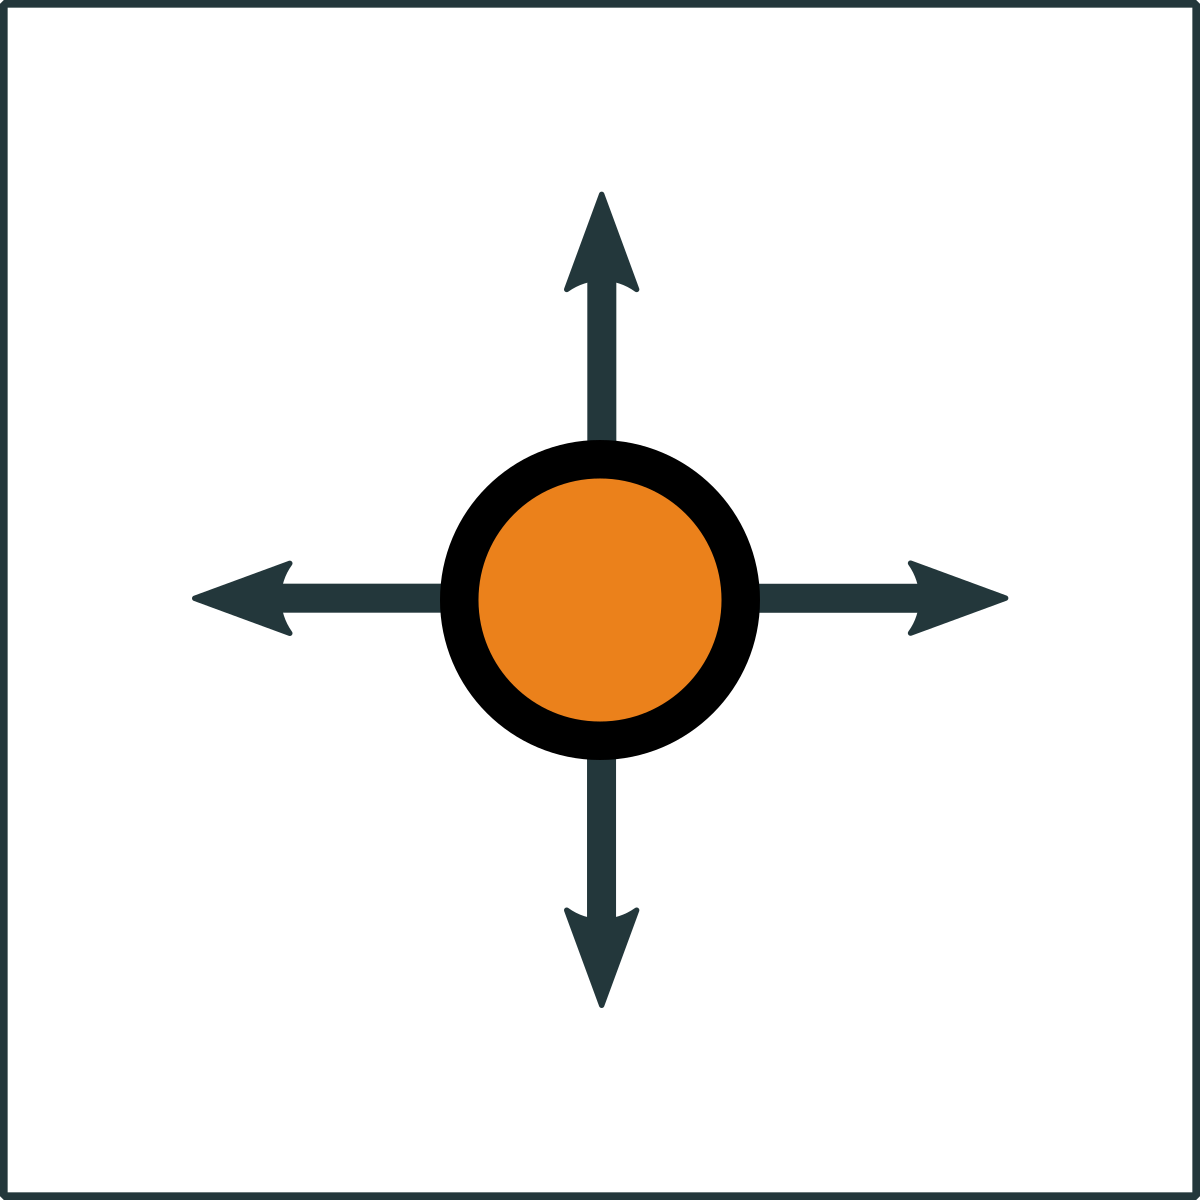
\includegraphics[width=0.5\textwidth]{img/agent-env-1.png}
  \end{center}
  \pause
  Model learning is the problem of estimating the dynamics of the system
  when we don't know it beforehand.
\end{frame}

\begin{frame}{Model learning}
  Formally, consider an agent in a system with state space $\mathcal{S}$
  with action space $\mathcal{A}$ with underlying dynamics 
  function $p(s_{t + 1} | s_t, a_t)$.

  We are interested in learning an approximate dynamics function
  \begin{align*}\hat{p}(s_{t + 1} | s_t, a_t)\end{align*}
  from a dataset of trajectories \begin{align*}\bm{\tau} = \{(s^{(i)}_0, a^{(i)}_0, s^{(i)}_1, a^{(i)}_1, \ldots, s^{(i)}_T)\}_{i = 1}^N\end{align*}
\end{frame}

\begin{frame}{Bayesian linear dynamical system}
  \pnote{Talk about conjugacy}
  A simple assumption: \textbf{Bayesian linear dynamical system} (LDS)
  \begin{alignat*}{3}
    \mu_{\isdmodel},\Sigma_{\isdmodel}&\sim\mathcal{NIW}(\Psi,\nu,\mu_0,\kappa)\,,~~~\dynmat,\dyncovar&&\sim\mathcal{MNIW}(\Psi,\nu,\bm{M}_0,\bm{V})\,,\\
    \state_0~|~\mu_{\isdmodel},\Sigma_{\isdmodel}&\sim\N(\mu_{\isdmodel}, \Sigma_{\isdmodel})\,,~~~~~\state_{t+1}~|~\state_t,\action_t&&\sim\N\left(\dynmat\begin{bmatrix}\state_t\\\action_t\end{bmatrix},\dyncovar\right) \textrm{ for } t \in [0,\ldots,\horizon]
  \end{alignat*}
  \pause
  \centering
  \includestandalone[width=0.5\textwidth]{tikz/blds}

  \pause
  We are interested in the posterior distribution 
  $
  p(\mu_\isdmodel, \Sigma_\isdmodel, \dynmat, \dyncovar | {s_0, a_0, \ldots, s_T})
  $
  which can be computed analytically.
\end{frame}

\begin{frame}{Variational inference at a high level}
  %For graphical models where we can't compute
  %the posterior analytically, \textbf{variational inference}
  %is a viable approach.

  \pause
  Consider a latent variable model with global variables
  $\theta$, local variables $z$ and observations $x$. Our desired
  posterior is $p(\theta, z | x)$

  \pause
  \textbf{Strategy}: convert inference into optimization
  \begin{itemize}
    \pause
  \item Instantiate \emph{variational distribution} $q_\phi(\theta, z)$
    where $\phi$ are free parameters
    \pause
  \item Define loss $\L[q_\phi(\theta, z)]
    \pause
  \item Minimize loss $\phi^* = \argmin_\phi \L[q_\phi(\theta, z)]
\end{itemize}
\pause
If $q(\theta, z)$ is sufficiently expressive,
it can approximate $p(\theta, z | x)$ quite well.
\end{frame}

%\begin{frame}{KL-divergence}
  %Kullback-Leibler (KL) divergence
  %is a measure of how far one probability distribution
  %is from another.

  %\pause
  %For distributions $q(x)$ and $p(x)$,
  %\begin{align*}
    %\textrm{KL}(q(x)\|p(x)) = \int q(x)\log \frac{q(x)}{p(x)}dx
  %\end{align*}

  %\pause
  %\textbf{Properties:}
  %\begin{itemize}
    %\item $\textrm{KL}(q(x)\|p(x)) = 0$ if $q(x) = p(x)$.
    %\item Asymmetric
  %\end{itemize}

%\end{frame}

\begin{frame}{Evidence lower bound}
  In general, we cannot even compute $KL(q(\theta, z)\|p(\theta, z | x))$
  because
  we don't know the posterior $p(\theta, z | x)$.

  \pause
  We can rewrite the KL divergence as
  \begin{align*}
    \KL(q(\theta, z)\|p(\theta, z|x)) &= \int q(\theta, z)\log\frac{q(\theta, z)}{p(\theta, z | x)}d\theta, z \\
    %&= \int q(\theta, z) \left(\log q(\theta, z) - \log p(\theta, z | x)\right)d\theta, z \\
    %&= \int q(\theta, z) \left(\log q(\theta, z) - \log \frac{p(\theta, z, x)}{p(x)}\right)d\theta, z \\
    %&= \int q(\theta, z) \left(\log q(\theta, z) - \log p(\theta, z, x) + \log p(x)\right)d\theta, z \\
                                      &= \log p(x) - \E_{q(\theta, z)}\left[\log\frac{p(x, \theta, z)}{q(\theta, z)}\right]
  \end{align*}

  \pause
  and maximize the \emph{evidence lower bound} (ELBO)
  \begin{align*}
    \L[q(\theta, z)] &= \E_{q(\theta, z)}\left[\log\frac{p(x, \theta, z)}{q(\theta, z)}\right]
  \end{align*}
\end{frame}

\begin{frame}{Variational inference for PGMs}
  For a general graphical model
  with variable set $\mathbf{X} = \{x_1, x_2, \ldots\}$
  we have joint distribution
  \begin{align*}
    p(\mathbf{X}) = \prod_i p(x_i | \textrm{pa}_i)
  \end{align*}
  where $\textrm{pa}_i$ are the parents of node $x_i$
  in the graph.

  \pause
  Let the set $\mathbf{H}$ be
  all unobserved variables and $\mathbf{V}$ be the observed.


  \pause
  We are interested in the posterior $p(\mathbf{H} | \mathbf{V})$
  and use variational distribution 
  \begin{align*}
    q(\mathbf{H}) = \prod_i q(\mathbf{H}_i)
  \end{align*}

  \pause
  This is called the \emph{mean-field} assumption.

\end{frame}

\begin{frame}{Variational inference for PGMs (cont.)}
  The ELBO is now
  \begin{align*}
    \L[q(\mathbf{H})] &= \E_{q(\mathbf{H})} \left[\log\frac{p(\mathbf{H}, \mathbf{V})}{q(\mathbf{H})}\right] \\
                      &= \int\prod_i q(\mathbf{H}_i) \left(\log p(\mathbf{H}, \mathbf{V}) - \log \prod_i q(\mathbf{H}_i)\right)d\mathbf{H}\\
                      &= \int q(\mathbf{H}_j) \left(\int \log p(\mathbf{H}, \mathbf{V})\prod_{i \neq j}q(\mathbf{H}_i)d\mathbf{H}_i \right)d\mathbf{H}_j \\&- \int q(\mathbf{H}_j)\log q(\mathbf{H}_j)d \mathbf{H}_j + \textrm{const.}\\
                      &= \int q(\mathbf{H}_j)\log \tilde{q}(\mathbf{H}_j, \mathbf{V})d \mathbf{H}_j- \int q(\mathbf{H}_j)\log q(\mathbf{H}_j)d \mathbf{H}_j  + \textrm{const.} \\
                      &= -\KL(q(\mathbf{H}_j)\|\tilde{q}(\mathbf{H}_j, \mathbf{V}))  + \textrm{const.}
  \end{align*}
  where 
  \begin{align*}
    \log\tilde{q}(\mathbf{H}_j, \mathbf{V}) = \E_{i \neq j}\left[\log p(\mathbf{H}, \mathbf{V})\right] + \textrm{const.}
  \end{align*}

\end{frame}

\begin{frame}{Optimizing a single factor}
  We can isolate a single factor for each hidden node in the graph $\mathbf{H}_j$.
  This makes optimizing a single variational factor easy!
  \pause
  \begin{align*}
    \L[q(\mathbf{H})] &= \KL(q(\mathbf{H}_j)\|\tilde{q}(\mathbf{H}_j, \mathbf{V}))  + \textrm{const.}
  \end{align*}
  \pause
  For a single factor $q(\mathbf{H}_j)$, this equation is minimized
  when $q(\mathbf{H}_j) = \tilde{q}(\mathbf{H}_j, \mathbf{V})$.

  \pause
  Furthermore, 
  \begin{align*}
    \log\tilde{q}(\mathbf{H}_j, \mathbf{V}) = \E_{i \neq j}\left[\log p(\mathbf{H}, \mathbf{V})\right] + \textrm{const.}
  \end{align*}
  is a function of only factors other than $q(\mathbf{H}_j)$  and observed data.

  \pause
  \metroset{block=fill}
  \begin{block}{Mean-field variational inference}
    Until converged,
    for each factor $q(\mathbf{H}_j)$,
    hold factors $q(\mathbf{H}_{i \neq j})$ constant and
    set $q(\mathbf{H}_j) = \tilde{q}(\mathbf{H}_j, \mathbf{V})$.
  \end{block}
\end{frame}

\begin{frame}{Conjugate-exponential graphical models}
  If our PGM is \emph{conjugate-exponential},
  where every node belongs in the exponential
  family of distributions, and is conjugate w.r.t. its parents,
  \begin{align*}
    \log\tilde{q}(\mathbf{H}_j, \mathbf{V}) = \E_{i \neq j}\left[\log p(\mathbf{H}, \mathbf{V})\right] + \textrm{const.}
  \end{align*}

  can be calculated in closed form!

  \pause
  An exponential family distribution is one that can be written in the following form:
  \begin{align*}
    p(x | \theta) = h(x) \exp \left\{\left\langle \eta_x(\theta), t_x(x)\right\rangle - \log Z(\eta(\theta))\right\}
  \end{align*}
  with 
  \begin{itemize}
    \pause
  \item $h(x)$: base measure
    \pause
  \item $\eta_x(\theta)$: natural parameter
    \pause
  \item $t_x(x)$: sufficient statistic
    \pause
  \item $\log Z(\eta_x(\theta))$: log-partition function
\end{itemize}
\end{frame}

\section{Structured variational autoencoder}


\begin{frame}{Model learning}
  Recall the model learning problem.
  \pause
  \begin{center}
    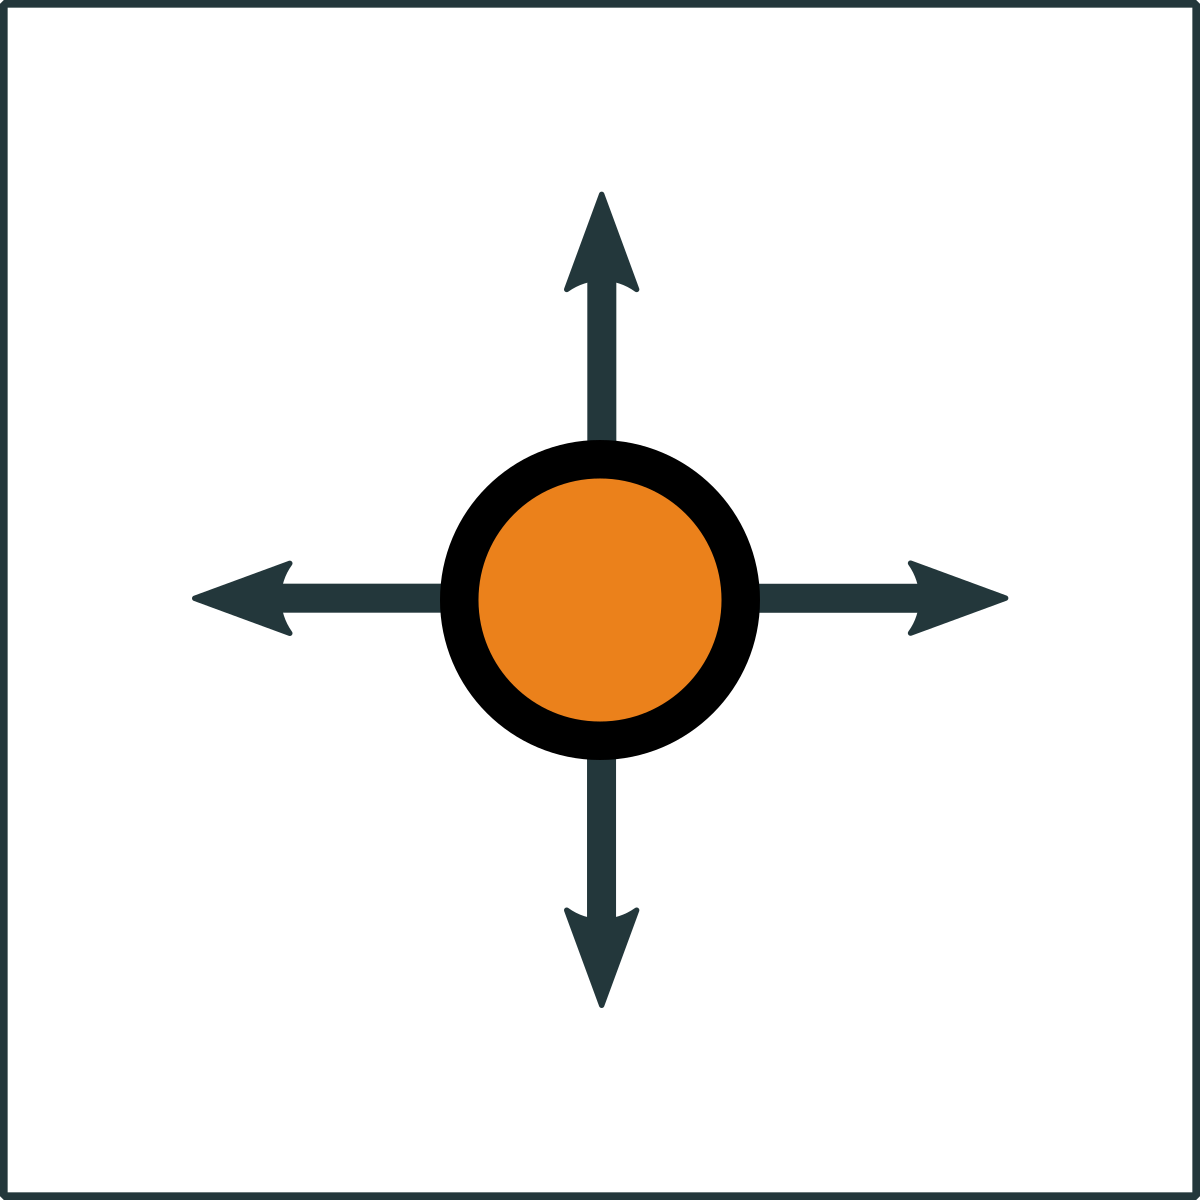
\includegraphics[width=0.3\textwidth]{img/agent-env-1.png}
  \end{center}

  \pause
  \centering
  \includestandalone[width=0.4\textwidth]{tikz/blds}
\end{frame}

\begin{frame}{Adding expressivity}
  One way of making the Bayesian LDS more expressive
  is to add a observation model.

  \pause

  \centering
  \includestandalone[width=0.4\textwidth]{tikz/lblds}

  \pause

  What if this observation model was a neural network?
\end{frame}

\begin{frame}{Structured variational autoencoder}
  We augment the Bayesian LDS with a neural network observation model.
  \pause
  \begin{alignat*}{3}
    \mu_{\isdmodel},\Sigma_{\isdmodel}&\sim\mathcal{NIW}(\Psi,\nu,\mu_0,\kappa)\,,~~~\dynmat,\dyncovar&&\sim\mathcal{MNIW}(\Psi,\nu,\bm{M}_0,\bm{V})\,,\label{eq:ldssvae-start}\\
    \latent_0~|~\mu_{\isdmodel},\Sigma_{\isdmodel}&\sim\N(\mu_{\isdmodel}, \Sigma_{\isdmodel})\,,~~~~~\latent_{t+1}~|~\latent_t,\action_t&&\sim\N\left(\dynmat\begin{bmatrix}\latent_t\\\action_t\end{bmatrix},\dyncovar\right) \textrm{ for } t \in [0,\ldots,\horizon]\,,\\
    \state_t~|~\latent_t&\sim\N\left(\mu_\gamma(\latent_t),\Sigma_\gamma(\latent_t)\right) \text{ for } t \in &&[0,\ldots,\horizon]
  \end{alignat*}
  where $\mu_\gamma(\latent_t)$ and $\Sigma_\gamma(\latent_t)$ are both neural networks parametrized by $\gamma$.
  This model is called a structured variational autoencoder (SVAE) \cite{svae}.

  \pause
  \textbf{But what does it do?}
\end{frame}

\begin{frame}{Inference in SVAE}
  First of all, a neural network is neither conjugate nor exponential.
  How do we perform inference?

  \pause
  \textbf{Strategy:} Run VMP, but use ``fake'' messages for the neural network observation model.

  \begin{center}
    \includegraphics<2>[width=0.15\textwidth]{img/vmp-svae-1}
    \includegraphics<3>[width=0.15\textwidth]{img/vmp-svae-2}
    \includegraphics<4>[width=0.15\textwidth]{img/vmp-svae-3}
  \end{center}

\end{frame}


\begin{frame}{Messages in SVAE}
  The message from a \textbf{non-conjugate, non-exponential family} observation $X$ to a parent $Y$ is
  \begin{align*}
    m_{X \rightarrow Y} = r_\xi(t_X(X))
  \end{align*}
  where $r_\xi$ is a neural network whose output
  is the same shape of a message from a conjugate-exponential child.

  \pause
  \metroset{block=fill}
  \begin{block}{Inference in a SVAE}
    \begin{enumerate}
      \item For a data $\tau = \{s_0, a_0, s_1, a_1, \ldots, s_T\}$,
        perform VMP using SVAE messages
      \item Compute the ELBO $\L[q(\{x_i\}_{i = 1}^T, \mu_{\isdmodel}, \Sigma_{\isdmodel}, \dynmat, \dyncovar)]$
      \item Update neural networks with $\nabla_{\gamma, \xi} \L[q(\{x_i\}_{i = 1}^T, \mu_{\isdmodel}, \Sigma_{\isdmodel}, \dynmat, \dyncovar)]$
      \item Update global parameters ($\mu_{\isdmodel}, \Sigma_{\isdmodel}, \dynmat, \dyncovar$) with natural gradients
    \end{enumerate}
  \end{block}
\end{frame}

\begin{frame}{Autoencoding}
  How is a SVAE an \emph{autoencoder}?

  \begin{center}
    \includestandalone[width=0.4\textwidth]{tikz/lblds}
  \end{center}

  \pause
  We have two neural networks:
  \begin{enumerate}
    \pause
  \item $r_\xi(s)$: recognition network, takes real data and ``encodes'' it
    \pause
  \item $\mu_\gamma(x), \Sigma_\gamma(x)$: observation network, takes latent data and ``decodes'' it
\end{enumerate}
\end{frame}

\section{Conclusion}

\subsection{Applications}
\begin{frame}{Why SVAE?}
  The SVAE naturally applies to scenarios where there is already a tractable PGM.

  \pause
  \begin{center}
    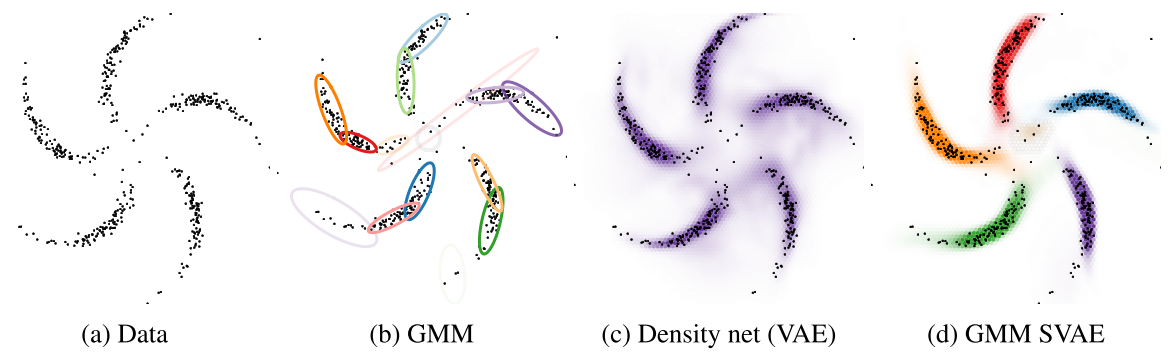
\includegraphics[frame,width=\textwidth]{img/svae-example}
  \end{center}

  \pause
  In this scenario, the SVAE enables modeling non-Gaussian cluster shapes \cite{svae}.
\end{frame}

\subsection{Current work}
\begin{frame}{Current work}
  One idea I am currently working on is using the SVAE to learn
  latent models to be used in reinforcement learning\footnotemark.

  \pause
  \textbf{General approach:}
  \begin{itemize}
    \item Learn a latent LDS
    \item Use MPC to control an agent in the latent space
  \end{itemize}

  \pause
  \textbf{Benefits of this approach:}
  \begin{itemize}
    \pause
  \item We can learn simple dynamics even with camera data
    \pause
  \item Model-based RL tends to be more sample efficient
    \pause
\end{itemize}
\pause
\alert{Demo}
\footnotetext[1]{Joint work with Marvin Zhang from UC Berkeley}
\end{frame}

\begin{frame}[standout]
  Questions?
\end{frame}

\appendix
\begin{frame}[allowframebreaks]{References}
  \bibliography{main}
  \bibliographystyle{unsrt}
\end{frame}


\end{document}
